\documentclass[11pt]{article}

% ACL review template. Change "review" to "final" for camera-ready or
% "preprint" for a non-anonymous version with page numbers.
\usepackage[review]{acl}

% Standard ACL package includes.
\usepackage{times}
\usepackage{latexsym}
\usepackage[T1]{fontenc}
\usepackage[utf8]{inputenc}
\usepackage{microtype}
\usepackage{inconsolata}

% Additional packages used by this survey.
\usepackage{booktabs}
\usepackage{graphicx}
\usepackage{array}
\usepackage{tabularx}
\usepackage{enumitem}
\usepackage{amsmath}
\usepackage{amsfonts}
\usepackage{amssymb}
\usepackage{forest}
\usepackage{tikz}
\usetikzlibrary{arrows.meta,calc}
\setlength{\emergencystretch}{3em}

% ACL review line numbers can drift visually toward the page center in dense
% two-column layouts. Keep them close to the text block edges.
\setlength{\linenumbersep}{6pt}

\title{Evidence Reliability and Action Control in Text-Based Retrieval-Augmented Generation:\\
A Structured Scoping Map and Agenda}

\author{Anonymous Authors}
\date{}

\begin{document}
\maketitle

\begin{abstract}
Text retrieval-augmented generation (RAG) grounds language models in external evidence, but retrieved evidence can be irrelevant, distracting, conflicting, stale, insufficient, or adversarially corrupted. This paper presents a structured scoping map and agenda for robust RAG under unreliable evidence, not a venue-complete systematic review or field census. We organize the literature around evidence reliability and action control: a robust RAG system should decide whether to retrieve, filter, re-rank, verify, answer, abstain, or ask for clarification. Our main contribution is a comparability framework: methods and benchmarks should only be compared when their failure type, evidence assumption, intervention point, metric target, and action policy are aligned. The synthesis is anchored in peer-reviewed or venue-linked evidence; a broader 268-paper final adjudicated evidence map is used as trend and audit evidence.
\end{abstract}

\section{Introduction}

Retrieval-augmented generation (RAG) combines a parametric language model with non-parametric evidence retrieved at inference time \citep{lewis2020rag}. The paradigm builds on earlier retrieval-augmented and open-domain QA work, and is now widely studied for document-grounded question answering, search, and assistant-style systems. RAG promises to reduce hallucination, update knowledge without retraining, and produce source-grounded answers. However, as RAG moves from curated benchmarks to open, mutable, and sometimes adversarial evidence sources, the retrieved evidence becomes a first-order source of risk.

The evidence used by a RAG system can fail in many ways. A retriever may return irrelevant passages, miss the positive passage, surface hard negatives, or rank stale evidence above fresh evidence. Even benign passages can distract a generator when they are topically similar but answer-irrelevant. Retrieved evidence may conflict with the model's parametric memory or with other retrieved sources. In open corpora, attackers may poison documents, manipulate dense retrieval, inject triggers, or exploit prompt templates. Finally, some queries are ambiguous, unsupported by the available corpus, or out of distribution; answering them requires calibrated control rather than forced generation.

These phenomena are often studied under separate names: noise robustness, context faithfulness, hallucination, knowledge conflict, corpus poisoning, indirect prompt injection, adaptive retrieval, uncertainty estimation, selective generation, and abstention. We argue that they are manifestations of one broader problem: \textbf{robust RAG under unreliable evidence}. A robust RAG system should not only maximize answer accuracy; it should estimate whether the evidence is reliable enough to answer and choose an appropriate action when it is not.

\paragraph{Differences from previous surveys.}
General RAG surveys summarize architectures, retrieval methods, and applications \citep{ragSurvey2024,ragComprehensive2025}. Evaluation surveys organize metrics and benchmarks \citep{ragEvaluationSurvey2024}. Trustworthy and secure RAG surveys cover broader axes such as privacy, fairness, accountability, safety, and explainability \citep{trustRAGCompass2024,trustworthyRAGSurvey2025,securityRAGSurvey2026}. These works provide valuable foundations, but they do not systematically center the end-to-end behavior of RAG when the retrieved evidence is unreliable. In contrast, this survey uses evidence unreliability as the organizing lens and connects retrieval noise, generator distraction, knowledge conflict, adversarial corruption, uncertainty, and calibration/control in one hierarchy.

\begin{table*}[t]
\centering
\scriptsize
\renewcommand{\arraystretch}{0.95}
\begin{tabularx}{\linewidth}{>{\raggedright\arraybackslash}p{0.19\linewidth}>{\raggedright\arraybackslash}p{0.22\linewidth}>{\raggedright\arraybackslash}p{0.20\linewidth}X}
\toprule
\textbf{Survey family} & \textbf{Main organizing unit} & \textbf{What it does not explain well} & \textbf{Increment of this survey} \\
\midrule
General RAG surveys \citep{ragSurvey2024,ragComprehensive2025} & Retriever/generator architectures, optimisation modules, applications & Why more retrieval can hurt; why relevance is insufficient; how evidence failure propagates to actions & Recasts RAG as evidence reliability plus action selection rather than architecture selection. \\
RAG evaluation surveys \citep{ragEvaluationSurvey2024} & Metrics, datasets, benchmark practice & Which metric corresponds to which failure mode and which system action & Links metrics to failure modes, intervention points, and action traces. \\
Trustworthy RAG surveys \citep{trustRAGCompass2024,trustworthyRAGSurvey2025} & Factuality, privacy, safety, fairness, transparency, accountability & How benign noise, conflict, attack, and uncertainty interact in one evidence state & Uses unreliable evidence as a single causal lens across trustworthiness dimensions. \\
RAG security surveys \citep{securityRAGSurvey2026,rrag134} & Attack surfaces, objectives, defenses, privacy risks & How adversarial corruption relates to non-adversarial noise, conflict, calibration, and abstention & Places security threats in the same failure--intervention matrix as benign reliability failures. \\
This survey & Evidence failure, intervention point, action policy, evaluation signal & -- & Provides a diagnostic schema: semantic fields must be compatible and claim-specific experimental controls must support the intended comparison. \\
\bottomrule
\end{tabularx}
\caption{Positioning relative to existing RAG surveys. Prior surveys provide broad architectural, evaluation, trustworthy, or security coverage; this survey uses unreliable evidence as the central lens and emphasizes how systems should act under evidence noise, conflict, corruption, and uncertainty.}
\label{tab:survey-comparison}
\end{table*}

\begin{table*}[t]
\centering
\scriptsize
\renewcommand{\arraystretch}{0.92}
\begin{tabularx}{\linewidth}{>{\raggedright\arraybackslash}p{0.18\linewidth}>{\raggedright\arraybackslash}p{0.26\linewidth}>{\raggedright\arraybackslash}p{0.25\linewidth}X}
\toprule
\textbf{Prior survey family} & \textbf{Common emphasis} & \textbf{Specific gap for robust-RAG comparison} & \textbf{Delta in this survey} \\
\midrule
General RAG surveys & Retrieval/generation architectures, optimisation modules, applications, and broad challenges. & Often treat robustness as a module or benchmark property, without separating evidence state from final answer policy. & Reframes robustness as evidence-state diagnosis plus action selection; distinguishes retrieve/filter/verify/answer/abstain as different outcomes. \\
RAG evaluation surveys & Metrics, datasets, automatic evaluation, and benchmark design. & Usually list metrics but do not force alignment between failure type, intervention point, and required action. & Adds an evaluation-assumption matrix and benchmark blueprint requiring evidence labels, action traces, cost, and threat-model fields. \\
Trustworthy RAG surveys & Factuality, privacy, fairness, safety, explainability, and accountability. & Broad trustworthiness axes can obscure whether the immediate failure is relevance, sufficiency, consistency, provenance, or integrity. & Uses evidence reliability dimensions to connect trustworthy-AI concerns to concrete RAG evidence failures. \\
Security-focused RAG surveys & Attack surfaces, defenses, privacy risks, poisoning, and prompt injection. & Security taxonomies can remain separate from benign noise, conflict, calibration, and answerability work. & Places adversarial corruption in the same failure--intervention matrix and normalizes attack/defense comparison by attacker capability. \\
Faithfulness / hallucination work & Unsupported generation, attribution, citation, and hallucination detection. & Correct answer, faithful citation, sufficient evidence, and calibrated abstention are often evaluated separately. & Separates answer accuracy, evidence support, citation faithfulness, confidence, and action quality; shows why improving one can worsen another. \\
\bottomrule
\end{tabularx}
\caption{Claim-level delta relative to adjacent survey families. The contribution is not broader coverage, but a comparison rule that changes how robustness, security, evaluation, and faithfulness claims are aligned.}
\label{tab:survey-delta}
\end{table*}


\begin{table*}[t]
\centering
\scriptsize
\renewcommand{\arraystretch}{0.9}
\begin{tabularx}{\linewidth}{>{\raggedright\arraybackslash}p{0.15\linewidth}>{\raggedright\arraybackslash}p{0.24\linewidth}>{\raggedright\arraybackslash}p{0.27\linewidth}X}
\toprule
\textbf{Overlapping work} & \textbf{Typical interpretation in adjacent surveys} & \textbf{Reinterpretation under evidence reliability + action control} & \textbf{Different conclusion enabled} \\
\midrule
RGB / RAG evaluation benchmarks & A benchmark measuring multiple RAG abilities. & A diagnostic split between noisy evidence, negative rejection, integration, and counterfactual evidence states. & A single RAG score hides which system action failed: ignore, integrate, reject, or expose conflict. \\
Irrelevant-context robustness & A robustness method or context-filtering problem. & A generator-selectivity failure conditioned on retrieved but harmful context. & It should not be compared directly with retriever training unless the intervention point and context hardness are fixed. \\
Sufficient Context / answerability work & An abstention or uncertainty benchmark. & A control-policy problem: evidence sufficiency determines answer vs re-retrieve vs abstain. & Abstention accuracy is incomplete without evidence sufficiency and action-cost labels. \\
PoisonedRAG / RAG poisoning & A security attack surface. & An integrity failure whose strength depends on corpus write access, retrieval success, generator access, and insertion budget. & Attack success rates are not comparable until capability fields are normalized. \\
RAGTruth / hallucination evaluation & A faithfulness or hallucination annotation resource. & A separation between answer correctness, claim support, citation support, and evidence sufficiency. & Correct answers can still fail evidence reliability; citation faithfulness and answer accuracy should be reported separately. \\
Self-RAG / adaptive retrieval & A retrieval-augmented generation method. & A system-control policy that chooses retrieve, critique, answer, or continue under uncertainty. & The relevant evaluation target is not only answer quality but whether the policy chose the right action at the right cost. \\
\bottomrule
\end{tabularx}
\caption{How the same papers are interpreted differently under the proposed framework. This table grounds the novelty claim in concrete reinterpretations rather than broad positioning statements.}
\label{tab:overlap-reinterpretation}
\end{table*}



Our novelty claim is therefore not that we cover every adjacent area more completely than prior surveys. It is that the evidence-reliability lens produces comparison rules that change how existing work should be interpreted. First, methods that all appear to address ``noise'' may intervene at retrieval, context construction, generator reasoning, or answer policy, so their scores should not be pooled. Second, adversarial-RAG results cannot be compared without attacker-capability normalization. Third, calibration, abstention, and adaptive retrieval are distinct control decisions, not interchangeable uncertainty metrics. These are the concrete insights used in the case studies and matrices below.

\paragraph{Contributions.}
This scoping map makes three bounded contributions.
\begin{enumerate}[leftmargin=*]
    \item \textbf{A decision procedure for comparability.} We specify how to align failure type, evidence assumption, intervention point, metric target, and action policy before comparing robust-RAG papers.
    \item \textbf{A tiered scoping evidence map.} We assemble 1,399 deduplicated candidates, a 100-paper core reading set, a 326-paper venue-augmented scoping set, and a 268-paper final adjudicated evidence map, while separating peer-reviewed backbone claims from preprint-heavy trends.
    \item \textbf{A research agenda for action-aware evaluation.} We derive attacker-capability and intervention matrices and give an action-trace benchmark blueprint as an agenda, not as a validated leaderboard.
\end{enumerate}

% Survey outline for Robust RAG. Top-down tree with live representative
% citations per leaf, using natbib aliases for compact rendering.

\definecolor{rragRootBd}{HTML}{2C3340}
\definecolor{rragLeafBg}{HTML}{F6F3EA}
\definecolor{rragLeafBd}{HTML}{C8C0B0}
\definecolor{rragBg}{HTML}{5B7393}  % background -- slate blue
\definecolor{rragEv}{HTML}{A06058}  % evidence -- muted brick
\definecolor{rragMd}{HTML}{5E8466}  % model -- forest sage
\definecolor{rragAt}{HTML}{8B6B91}  % adversarial -- plum
\definecolor{rragCt}{HTML}{4D8786}  % control -- teal
\definecolor{rragFu}{HTML}{A98552}  % future/guidelines -- ochre

% Compact aliases keep the outline readable while preserving live citations.
\defcitealias{lewis2020rag}{RAG}
\defcitealias{ragSurvey2024}{RAG-Survey}
\defcitealias{ragComprehensive2025}{RAG-Frontiers}
\defcitealias{ragEvaluationSurvey2024}{Eval-Survey}
\defcitealias{trustRAGCompass2024}{Trust-Compass}
\defcitealias{trustworthyRAGSurvey2025}{Trustworthy-RAG}
\defcitealias{securityRAGSurvey2026}{Secure-RAG}
\defcitealias{irrelevantContext2023}{IrrelCtx}
\defcitealias{raat2024}{RAAT}
\defcitealias{rgb2023}{RGB}
\defcitealias{ragTruth2024}{RAGTruth}
\defcitealias{queryRobustness2025}{QueryRobust}
\defcitealias{chainOfNote2023}{CoN}
\defcitealias{sufficientContext2024}{SuffCtx}
\defcitealias{tugOfWar2024}{Tug-of-War}
\defcitealias{faithfulRAG2025}{FaithfulRAG}
\defcitealias{astuteRAG2025}{AstuteRAG}
\defcitealias{poisoningRetrievalCorpora2023}{PoisonRetr}
\defcitealias{poisonedRAG2024}{PoisonedRAG}
\defcitealias{badRAG2024}{BadRAG}
\defcitealias{trojanRAG2024}{TrojanRAG}
\defcitealias{phantom2024}{Phantom}
\defcitealias{aip2025}{AIP}
\defcitealias{certifiedRAG2024}{RobustRAG}
\defcitealias{selfRAG2023}{Self-RAG}
\defcitealias{whenToRetrieve2024}{Adapt-LLM}
\defcitealias{ctrla2025}{CtrlA}
\defcitealias{crag2024}{CRAG}
\defcitealias{calibRAG2025}{CalibRAG}
\defcitealias{uncertaintyRAG2024}{UncertaintyRAG}
% --- rrag aliases ---
\defcitealias{rrag001}{URAG}
\defcitealias{rrag002}{SABER}
\defcitealias{rrag003}{FirstDrop}
\defcitealias{rrag004}{ProGRank}
\defcitealias{rrag005}{RetrBarrier}
\defcitealias{rrag006}{OverSearch}
\defcitealias{rrag007}{NAACL-Cal}
\defcitealias{rrag008}{CoRect}
\defcitealias{rrag009}{CleanBase}
\defcitealias{rrag010}{AdvCoT}
\defcitealias{rrag011}{SparseAtt-Def}
\defcitealias{rrag012}{UE-Axioms}
\defcitealias{rrag013}{TrustRAG}
\defcitealias{rrag014}{PoisonTrace}
\defcitealias{rrag015}{AVFilter}
\defcitealias{rrag016}{SecureRAG-Def}
\defcitealias{rrag017}{SeCon-RAG}
\defcitealias{rrag018}{GMTP}
\defcitealias{rrag019}{SafeRAG}
\defcitealias{rrag020}{Rescue-Unp}
\defcitealias{rrag021}{ReliabilityRAG}
\defcitealias{rrag023}{PoisonArena}
\defcitealias{rrag024}{ParamMute}
\defcitealias{rrag027}{MagicMushroom}
\defcitealias{rrag028}{MIRAGE}
\defcitealias{rrag029}{MAGIC}
\defcitealias{rrag030}{DontKnow}
\defcitealias{rrag031}{DRAGged}
\defcitealias{rrag032}{CUB}
\defcitealias{rrag033}{Poison-Bench}
\defcitealias{rrag034}{AdaRetr-Bench}
\defcitealias{rrag035}{LIAR}
\defcitealias{rrag036}{WikiContradict}
\defcitealias{rrag037}{RobustRALM}
\defcitealias{rrag038}{Trust-Or-Not}
\defcitealias{rrag039}{LC-RAG}
\defcitealias{rrag040}{FaithEval}
\defcitealias{rrag041}{Counterfactual}
\defcitealias{rrag042}{Context-DPO}
\defcitealias{rrag043}{Gullible}
\defcitealias{rrag044}{FILCO}
\defcitealias{rrag045}{KnowBoundary}
\defcitealias{rrag046}{Chameleon}
\defcitealias{rrag051}{GraphRAG-Fire}
\defcitealias{rrag055}{WorseZS}
\defcitealias{rrag058}{UDCG}
\defcitealias{rrag064}{UQ-Reason}
\defcitealias{rrag066}{Divide-Align}
\defcitealias{rrag073}{Denoise-First}
\defcitealias{rrag077}{ERA}
\defcitealias{rrag087}{Merlin-RAG}
\defcitealias{rrag088}{ProbeRAG}
\defcitealias{rrag092}{AfterRetr}
\defcitealias{rrag093}{SURE-RAG}
\defcitealias{rrag095}{BalanceRAG}
\defcitealias{rrag105}{FaithUQ}
\defcitealias{rrag107}{DeRAG}
\defcitealias{rrag111}{Unanswerability}
\defcitealias{rrag112}{RealConflict}
\defcitealias{rrag115}{RAFT}
\defcitealias{rrag127}{GraphPoison}
\defcitealias{rrag128}{Traceback}
\defcitealias{rrag131}{DistrAware}
\defcitealias{rrag132}{SourcePref}
\defcitealias{rrag134}{Secure-Survey}
\defcitealias{rrag136}{Curse-Help}
\defcitealias{rrag141}{MTRAG-UN}
\defcitealias{rrag143}{LostInEvi}
\defcitealias{rrag153}{Decide-Retr}
\defcitealias{rrag154}{SLM-Use}
\defcitealias{rrag174}{CARE-RAG}
\defcitealias{rrag175}{StylePoison}
\defcitealias{rrag180}{PrismRAG}
\defcitealias{rrag182}{PKV-Fusion}
\defcitealias{rrag183}{PRGB}
\defcitealias{rrag193}{CRUMQs}
\defcitealias{rrag200}{END-Drop}
\defcitealias{rrag201}{DynContext}
\defcitealias{rrag206}{DSSP-RAG}
\defcitealias{rrag214}{Parenting}
\defcitealias{rrag219}{RAGE-ICL}
\defcitealias{rrag226}{RECOMP}
\defcitealias{rrag229}{MM-RAG-Risk}

\begin{figure*}[!t]
\vspace*{-0.35cm}%
\setlength{\abovecaptionskip}{4pt}%
\centering
\makebox[\textwidth][c]{%
\hspace*{-0.30cm}%
\begin{tikzpicture}[
  x=1cm,y=1cm,
  root/.style={
    draw=rragRootBd, fill=white, text=rragRootBd,
    rounded corners=2pt, line width=0.7pt,
    font=\tiny\bfseries, align=center,
    inner xsep=5pt, inner ysep=4pt, text width=4.35cm
  },
  branch/.style={
    draw=#1, fill=#1, text=white,
    rounded corners=2pt, line width=0pt,
    font=\tiny\bfseries, align=center,
    inner xsep=3pt, inner ysep=3pt, text width=2.22cm
  },
  leaf/.style={
    draw=rragLeafBd, fill=rragLeafBg, text=black!84,
    rounded corners=1.5pt, line width=0.25pt,
    font=\fontsize{4.4}{4.75}\selectfont, align=left,
    inner xsep=1.9pt, inner ysep=1.4pt, text width=2.66cm
  },
  link/.style={-Latex, line width=0.4pt, color=black!42},
  twig/.style={line width=0.35pt, color=black!38, rounded corners=2pt}
]
\newcommand{\leafGap}{6pt}

\node[root] (root) at (0,0) {\textsc{Robust RAG}\\\textsc{under Unreliable Evidence}};

\node[branch=rragBg] (b1) at (-8.50,-1.12) {\S1--\S2\\Background \&\\Taxonomy};
\node[branch=rragEv] (b2) at (-5.10,-1.12) {\S3\\Evidence-Centric\\Robustness};
\node[branch=rragMd] (b3) at (-1.70,-1.12) {\S4\\Model-Centric\\Robustness};
\node[branch=rragAt] (b4) at (1.70,-1.12) {\S5\\Adversarial\\Corruption};
\node[branch=rragCt] (b5) at (5.10,-1.12) {\S6--\S7\\Control \&\\Evaluation};
\node[branch=rragFu] (b6) at (8.50,-1.12) {\S8--\S11\\Synthesis,\\Guidelines \&\\Future};

\coordinate (rootFork) at (0,-0.62);
\draw[twig] (root.south) -- (rootFork);
\draw[twig] (rootFork -| b1.north) -- (rootFork -| b6.north);
\foreach \b in {b1,b2,b3,b4,b5,b6} {
  \draw[link] (rootFork -| \b.north) -- (\b.north);
}

% =============== Background and taxonomy ===============
\node[leaf] (b1l1) at (-8.50,-2.55) {\textbf{\S1~Problem framing}\\RAG as evidence-conditioned policy; running example\\{\color{black!62}\citetalias{lewis2020rag}, \citetalias{ragSurvey2024}, \citetalias{ragComprehensive2025}, \citetalias{trustRAGCompass2024}, \citetalias{trustworthyRAGSurvey2025}, \citetalias{rrag037}, \citetalias{queryRobustness2025}, \citetalias{rgb2023}}};
\node[leaf] (b1l2) at (-8.50,-4.20) {\textbf{Evidence reliability}\\relevance, sufficiency, faithfulness, consistency, integrity\\{\color{black!62}\citetalias{irrelevantContext2023}, \citetalias{sufficientContext2024}, \citetalias{tugOfWar2024}, \citetalias{faithfulRAG2025}, \citetalias{poisonedRAG2024}, \citetalias{badRAG2024}, \citetalias{rrag003}, \citetalias{rrag045}}};
\node[leaf] (b1l3) at (-8.50,-5.85) {\textbf{\S2~Comparability tuple}\\evidence-, model-, system-centric, evaluation layers\\{\color{black!62}\citetalias{trustRAGCompass2024}, \citetalias{trustworthyRAGSurvey2025}, \citetalias{ragComprehensive2025}, \citetalias{ragEvaluationSurvey2024}, \citetalias{securityRAGSurvey2026}, \citetalias{rrag073}, \citetalias{rrag134}, \citetalias{ragSurvey2024}}};
\node[leaf] (b1l4) at (-8.50,-7.50) {\textbf{Operational pipeline}\\detect, diagnose, mitigate, control, monitor\\{\color{black!62}\citetalias{chainOfNote2023}, \citetalias{crag2024}, \citetalias{sufficientContext2024}, \citetalias{selfRAG2023}, \citetalias{ctrla2025}, \citetalias{calibRAG2025}, \citetalias{rrag002}, \citetalias{astuteRAG2025}}};

% =============== Evidence-centric (Section 4) ===============
\node[leaf] (b2l1) at (-5.10,-2.55) {\textbf{Noisy retrieval}\\irrelevant passages, hard negatives, missing positives\\{\color{black!62}\citetalias{irrelevantContext2023}, \citetalias{raat2024}, \citetalias{rgb2023}, \citetalias{rrag027}, \citetalias{rrag001}, \citetalias{rrag037}, \citetalias{rrag043}, \citetalias{rrag055}, \citetalias{rrag030}}};
\node[leaf] (b2l2) at (-5.10,-4.20) {\textbf{Distraction}\\negative context utility, ordering, long-context erosion\\{\color{black!62}\citetalias{rrag003}, \citetalias{rrag032}, \citetalias{rrag039}, \citetalias{rrag058}, \citetalias{rrag131}, \citetalias{rrag136}, \citetalias{rrag143}, \citetalias{rrag180}, \citetalias{rrag200}, \citetalias{rrag201}}};
\node[leaf] (b2l3) at (-5.10,-5.85) {\textbf{Query- \& index-side noise}\\query perturbation, chunking, hybrid retrieval, multimodality\\{\color{black!62}\citetalias{queryRobustness2025}, \citetalias{rrag073}, \citetalias{rrag141}, \citetalias{rrag051}, \citetalias{rrag127}, \citetalias{rrag175}, \citetalias{rrag229}, \citetalias{rrag182}}};
\node[leaf] (b2l4) at (-5.10,-7.50) {\textbf{Evidence-side controls}\\filtering, reranking, compression, query repair\\{\color{black!62}\citetalias{rrag044}, \citetalias{rrag226}, \citetalias{rrag092}, \citetalias{rrag004}, \citetalias{rrag017}, \citetalias{rrag154}, \citetalias{rrag020}, \citetalias{rrag073}}};

% =============== Model-centric (Section 5) ===============
\node[leaf] (b3l1) at (-1.70,-2.55) {\textbf{Context utilization}\\notes, filtering, claim-level support, intermediate reasoning\\{\color{black!62}\citetalias{chainOfNote2023}, \citetalias{rrag032}, \citetalias{rrag115}, \citetalias{rrag226}, \citetalias{rrag088}, \citetalias{rrag042}, \citetalias{rrag038}, \citetalias{rrag040}}};
\node[leaf] (b3l2) at (-1.70,-4.20) {\textbf{Knowledge conflict}\\parametric vs.\ retrieved, retrieved vs.\ retrieved, sources\\{\color{black!62}\citetalias{tugOfWar2024}, \citetalias{faithfulRAG2025}, \citetalias{astuteRAG2025}, \citetalias{rrag008}, \citetalias{rrag024}, \citetalias{rrag029}, \citetalias{rrag031}, \citetalias{rrag036}, \citetalias{rrag112}, \citetalias{rrag174}}};
\node[leaf] (b3l3) at (-1.70,-5.85) {\textbf{Faithful generation \& attribution}\\citations, verification, source reliability, hallucination\\{\color{black!62}\citetalias{ragTruth2024}, \citetalias{rrag206}, \citetalias{rrag132}, \citetalias{rrag115}, \citetalias{rrag017}, \citetalias{rrag013}, \citetalias{rrag045}, \citetalias{rrag046}, \citetalias{rrag092}}};
\node[leaf] (b3l4) at (-1.70,-7.50) {\textbf{Limits of model-centric fixes}\\suppression vs.\ trust, situated faithfulness, robust training\\{\color{black!62}\citetalias{rrag024}, \citetalias{rrag038}, \citetalias{rrag042}, \citetalias{rrag043}, \citetalias{rrag214}, \citetalias{rrag112}, \citetalias{rrag066}, \citetalias{rrag077}}};

% =============== Adversarial corruption (Section 6) ===============
\node[leaf] (b4l1) at (1.70,-2.55) {\textbf{Corpus poisoning \& backdoors}\\malicious passages, triggers, knowledge corruption\\{\color{black!62}\citetalias{poisoningRetrievalCorpora2023}, \citetalias{poisonedRAG2024}, \citetalias{badRAG2024}, \citetalias{trojanRAG2024}, \citetalias{phantom2024}, \citetalias{rrag010}, \citetalias{rrag028}, \citetalias{rrag035}, \citetalias{rrag175}, \citetalias{rrag127}}};
\node[leaf] (b4l2) at (1.70,-4.20) {\textbf{Prompt-level \& injection attacks}\\indirect injection, template attacks, agent attacks\\{\color{black!62}\citetalias{aip2025}, \citetalias{rrag005}, \citetalias{rrag107}, \citetalias{rrag019}, \citetalias{rrag051}, \citetalias{rrag023}, \citetalias{rrag033}, \citetalias{rrag214}}};
\node[leaf] (b4l3) at (1.70,-5.85) {\textbf{Defense-in-depth}\\sanitization, robust retrieval, attention filters, traceback\\{\color{black!62}\citetalias{certifiedRAG2024}, \citetalias{rrag004}, \citetalias{rrag009}, \citetalias{rrag011}, \citetalias{rrag013}, \citetalias{rrag014}, \citetalias{rrag015}, \citetalias{rrag016}, \citetalias{rrag018}, \citetalias{rrag020}, \citetalias{rrag021}, \citetalias{rrag128}}};
\node[leaf] (b4l4) at (1.70,-7.50) {\textbf{Threat models \& attack realism}\\attacker knowledge, retrieval realism, stealth, benchmarks\\{\color{black!62}\citetalias{rrag005}, \citetalias{rrag019}, \citetalias{rrag023}, \citetalias{rrag033}, \citetalias{rrag028}, \citetalias{rrag015}, \citetalias{securityRAGSurvey2026}, \citetalias{rrag134}}};

% =============== Control and evaluation (Sections 7-8) ===============
\node[leaf] (b5l1) at (5.10,-2.55) {\textbf{Adaptive retrieval}\\when to retrieve, re-retrieve, stop, decompose\\{\color{black!62}\citetalias{selfRAG2023}, \citetalias{whenToRetrieve2024}, \citetalias{ctrla2025}, \citetalias{crag2024}, \citetalias{rrag006}, \citetalias{rrag034}, \citetalias{rrag153}, \citetalias{rrag066}, \citetalias{rrag077}}};
\node[leaf] (b5l2) at (5.10,-4.20) {\textbf{Calibration, abstention \& uncertainty}\\confidence, refusal, clarification, conformal control\\{\color{black!62}\citetalias{calibRAG2025}, \citetalias{uncertaintyRAG2024}, \citetalias{rrag002}, \citetalias{rrag007}, \citetalias{rrag012}, \citetalias{rrag041}, \citetalias{rrag064}, \citetalias{rrag087}, \citetalias{rrag095}, \citetalias{rrag105}, \citetalias{rrag111}, \citetalias{rrag141}, \citetalias{rrag193}}};
\node[leaf] (b5l3) at (5.10,-5.85) {\textbf{Policy composition \& cost-aware control}\\over-retrieval, cost--latency budgets, escalation, interaction\\{\color{black!62}\citetalias{rrag006}, \citetalias{rrag034}, \citetalias{rrag111}, \citetalias{rrag141}, \citetalias{rrag041}, \citetalias{rrag002}, \citetalias{rrag066}, \citetalias{rrag038}}};
\node[leaf] (b5l4) at (5.10,-7.50) {\textbf{Evaluation \& benchmarks}\\noise, conflict, attacks, selective risk, action quality\\{\color{black!62}\citetalias{rgb2023}, \citetalias{ragTruth2024}, \citetalias{queryRobustness2025}, \citetalias{rrag001}, \citetalias{rrag019}, \citetalias{rrag023}, \citetalias{rrag027}, \citetalias{rrag029}, \citetalias{rrag036}, \citetalias{rrag040}, \citetalias{rrag093}, \citetalias{rrag183}}};

% =============== Synthesis / guidelines / future (Sections 9-12) ===============
\node[leaf] (b6l1) at (8.50,-2.55) {\textbf{Design principles}\\evidence as constructed context, source reliability, action quality\\{\color{black!62}\citetalias{rrag058}, \citetalias{rrag132}, \citetalias{rrag111}, \citetalias{sufficientContext2024}, \citetalias{astuteRAG2025}, \citetalias{chainOfNote2023}, \citetalias{calibRAG2025}, \citetalias{rrag038}}};
\node[leaf] (b6l2) at (8.50,-4.20) {\textbf{Cross-cutting analysis}\\intervention points, method families, Pareto progress\\{\color{black!62}\citetalias{irrelevantContext2023}, \citetalias{chainOfNote2023}, \citetalias{sufficientContext2024}, \citetalias{certifiedRAG2024}, \citetalias{rrag004}, \citetalias{rrag013}, \citetalias{astuteRAG2025}, \citetalias{ragComprehensive2025}}};
\node[leaf] (b6l3) at (8.50,-5.85) {\textbf{Practical guidelines}\\for benchmark builders, method designers, system builders\\{\color{black!62}\citetalias{rrag019}, \citetalias{rrag023}, \citetalias{rrag027}, \citetalias{rrag033}, \citetalias{rrag034}, \citetalias{rrag141}, \citetalias{rrag193}, \citetalias{certifiedRAG2024}, \citetalias{rrag013}, \citetalias{rrag017}}};
\node[leaf] (b6l4) at (8.50,-7.50) {\textbf{Open challenges \& future}\\joint benchmarks, agentic/multimodal RAG, versioned maps\\{\color{black!62}\citetalias{rrag051}, \citetalias{rrag127}, \citetalias{rrag175}, \citetalias{rrag229}, \citetalias{rrag219}, \citetalias{trustworthyRAGSurvey2025}, \citetalias{securityRAGSurvey2026}, \citetalias{rrag134}}};

\foreach \b/\last in {b1/b1l4,b2/b2l4,b3/b3l4,b4/b4l4,b5/b5l4,b6/b6l4} {
  \coordinate (\b fork) at ($(\b.south)+(0,-0.18)$);
  \draw[twig] (\b.south) -- (\b fork) -| ([xshift=\leafGap]\last.east);
}
\foreach \l in {b1l1,b1l2,b1l3,b1l4,b2l1,b2l2,b2l3,b2l4,b3l1,b3l2,b3l3,b3l4,b4l1,b4l2,b4l3,b4l4,b5l1,b5l2,b5l3,b5l4,b6l1,b6l2,b6l3,b6l4} {
  \draw[link] ([xshift=\leafGap]\l.east) -- (\l.east);
}

\end{tikzpicture}%
}
\caption{\textbf{Outline of this paper.} A top-down view of the paper structure. The root problem is robust RAG under unreliable evidence; the paper then moves from background and taxonomy to evidence-centric, model-centric, adversarial, system-control, evaluation, synthesis, and future-facing guidelines. Each leaf lists representative cited work using compact aliases.}
\label{fig:survey_outline}
\end{figure*}

\begin{table*}[t]
\centering
\scriptsize
\renewcommand{\arraystretch}{0.95}
\begin{tabularx}{\linewidth}{>{\raggedright\arraybackslash}p{0.24\linewidth}>{\raggedright\arraybackslash}p{0.18\linewidth}>{\raggedright\arraybackslash}p{0.25\linewidth}X}
\toprule
\textbf{Claim type} & \textbf{Evidence stratum} & \textbf{What we claim} & \textbf{What we do not claim} \\
\midrule
Established RAG failure mechanisms & Peer-reviewed or venue-linked anchors plus repeated preprints & Irrelevant, insufficient, conflicting, and misleading retrieved context can change answers, confidence, and attribution in text QA/document-grounded RAG. & That every deployment domain exhibits the same frequency, cost, or mitigation effectiveness. \\
Security and poisoning landscape & Mostly emerging preprints with a small number of venue-linked security/NLP papers & RAG attacks differ sharply by corpus write access, query control, retriever visibility, and generator access; attack success rates are not comparable without these fields. & That the attack distribution in the evidence map is a peer-reviewed consensus about real-world incident prevalence. \\
Corpus-level distribution findings & The canonical 342-row adjudicated Map B plus source-strata metadata & The current mapped corpus is still uneven across failure modes and source strata despite stronger venue coverage. & That the counts are a complete census of all IR, NLP, security, or ML proceedings. \\
Action-control benchmark proposal & Synthesis from existing benchmarks and control/calibration papers & Future robust-RAG benchmarks should score evidence state, final answer, and system action jointly. & That our blueprint is already a validated leaderboard or that one metric can summarize robustness. \\
Design guidance & Risk-analysis extrapolation from text/document-grounded RAG evidence & Higher-risk systems should expose provenance, conflict, uncertainty, and abstention/escalation pathways. & That the evidence map directly validates enterprise, medical, legal, multimodal, or agentic deployments. \\
\bottomrule
\end{tabularx}
\caption{Claim-strength tiers used in this survey. We separate peer-reviewed or venue-linked evidence, emerging preprint trends, corpus-derived observations, and design hypotheses so that a preprint-heavy map is not mistaken for settled consensus.}
\label{tab:claim-strength}
\end{table*}


\paragraph{Scope and target readers.}
The target readers are RAG benchmark builders, method designers, and system builders who need to decide how to evaluate text and document-grounded RAG under unreliable evidence. We do not attempt to replace broad RAG architecture surveys, trustworthy AI surveys, security-only surveys, or historical reviews of IR/open-domain QA. We also do not claim venue-complete coverage. Instead, we ask a narrower question: when evidence is unreliable, what failure is present, where can a method intervene, what assumptions does it make, what metric can evaluate it, and what action should the system take? Multilingual, multimodal, code, tool-using, and agentic RAG are treated as boundary areas: they appear when they directly affect evidence reliability, but they are excluded from the empirical backbone because their evidence objects and action spaces differ from text/document-grounded RAG.

\section{Framework First: Decision Procedure and Re-analysis Pilot}
\label{sec:framework-first}

\begin{table*}[t]
\centering
\scriptsize
\renewcommand{\arraystretch}{0.88}
\begin{tabularx}{\linewidth}{>{\raggedright\arraybackslash}p{0.13\linewidth}>{\raggedright\arraybackslash}p{0.26\linewidth}>{\raggedright\arraybackslash}p{0.30\linewidth}X}
\toprule
\textbf{Coordinate} & \textbf{Controlled values} & \textbf{Equivalence / boundary rule} & \textbf{Verdict effect} \\
\midrule
Evidence state & Supported; irrelevant/distracting; insufficient; conflicting; stale/weak provenance; adversarially manipulated; not evidence-conditioned. & Code what is observable at the decision boundary. Query ambiguity, OOD input, confidence, and attacker access are not evidence states by themselves. & A direct performance claim normally requires a common state or an explicit cross-state estimand. \\
Origin / capability & Benign retrieval; constructed stressor; natural conflict/drift; query or distribution shift; attacker-created evidence; shared clean harness. & Record how the state arose. For security, include corpus write access, query control, retriever visibility, generator access, insertion budget, objective, and target. & A cross-source rank over two different games narrows at best and is otherwise undefined; a shared harness may deliberately vary capability as the controlled factor. \\
Intervention point & Corpus/index; retriever; reranker; context assembly/compression; generator prompting or training; verifier; system-control policy; evaluation-only artifact. & Code the component changed. Different interventions may be compared as alternatives when a shared end-to-end harness controls the remaining pipeline; otherwise they provide component-specific or compositional evidence. & C3 never enters the decision rule. Comparing two different systems means the intervention differs, so a C3 mismatch is the normal state of a comparison and cannot by itself make one undefined; it is recorded so a reader knows what changed. \\
Outcome / unit & Answer correctness; retrieval quality; evidence support; attack or defense utility; privacy leakage; calibration; selective risk/coverage; cost/latency; human preference. & Record definition, direction, aggregation, and unit. Relative gains over different baselines are not automatically a shared estimand. & A one-scalar ranking requires a common target. Without one there is no operating point to re-read at, so the gap is undefined rather than narrowed. \\
Policy / utility & Answer; abstain; re-retrieve; filter; verify; expose conflict; clarify; quarantine; recover; not applicable; unreported. & Use \emph{not applicable} for fixed descriptive comparisons. When policies compete, report action set, stakes, preferences, coverage, and cost. & Different actions can be ranked only under common utility; a signal alone does not establish the preferred response. A stated price at the other side's setting narrows the comparison. \\
Second-stage controls & Dataset/corpus snapshot; retriever/top-$k$/chunking; generator/decoding; compute budget; baselines; uncertainty/statistical design. & Select controls according to the stated inference. The tuple cannot remove confounding from unmatched experimental systems. & Tuple compatibility is necessary diagnostic information but not sufficient for a direct empirical ranking. \\
Final verdict & Survives; narrows; undefined. & Exactly the rule of \S\ref{sec:estimands}, and the only verdict vocabulary used anywhere in this paper or its artifacts. \emph{Survives}: C1, C2, C4 and C5 all match, so the quoted gap stands. \emph{Narrows}: a threatening coordinate differs but a side reports an operating point at the other's setting, or the comparison holds on a strict subset; report that matched number. \emph{Undefined}: no such operating point exists, or a decision-critical field is unavailable after full-text inspection. & Verdicts attach to comparison claims, not permanently to paper pairs, and a new shared-harness experiment can change the supported verdict. An undefined comparison is never replaced by a substitute number computed across the unmatched coordinate. \\
\bottomrule
\end{tabularx}
\caption{The decision procedure of \S\ref{sec:estimands} in full. The five coordinates diagnose semantic compatibility and claim-specific controls determine whether the claim as written is warranted, but only C1, C2, C4 and C5 enter the verdict: C3 is the thing being compared and is recorded rather than tested. The three verdicts here are the same three used in the body, the census codebook and every released artifact.}
\label{tab:framework-decision-procedure}
\end{table*}

\begin{table*}[t]
\centering
\tiny
\renewcommand{\arraystretch}{0.86}
\begin{tabularx}{\linewidth}{>{\raggedright\arraybackslash}p{0.13\linewidth}>{\raggedright\arraybackslash}p{0.16\linewidth}>{\raggedright\arraybackslash}p{0.14\linewidth}>{\raggedright\arraybackslash}p{0.10\linewidth}>{\raggedright\arraybackslash}p{0.18\linewidth}X}
\toprule
\textbf{Naive comparison} & \textbf{Tuple summary (F/A/I/M/Act)} & \textbf{Breaking coordinate(s)} & \textbf{Verdict} & \textbf{What a valid comparison would require} & \textbf{Changed interpretation} \\
\midrule
IrrelCtx vs. RAAT vs. RGB as ``noise robustness'' & Shared relevance/noise; benign or benchmark stressors; generator sensitivity vs. training vs. benchmark; accuracy/ability metrics; action mostly unreported. & Intervention, metric, action. & Partial / under-specified & Fix negative type, rank, gold-evidence availability, generator, metric family, and explicit answer/abstain policy. & They map different operating regions: generator selectivity, noise-aware training, and diagnostic benchmark design. \\
Context filtering vs. Chain-of-Note as distraction mitigation & Shared distraction; benign context noise; context assembly vs. generator reasoning; answer robustness; answer action implicit. & Intervention and action. & Partial & Evaluate both on the same retrieved contexts with the same generator, answer policy, and evidence-support metric. & A filter and a reasoning prompt can compose; ranking them as substitutes hides pipeline position. \\
Sufficient Context vs. Self-RAG as control & Sufficiency vs. retrieval-need uncertainty; benign missing evidence; sufficiency predictor vs. learned retrieve/critique policy; selective risk vs. utility/cost; abstain vs. retrieve/answer. & Failure, intervention, metric, action. & Partial & Hold evidence-sufficiency labels fixed and score the same action set: answer, abstain, retrieve, or critique. & One estimates whether evidence is enough; the other learns a broader control policy. \\
Calibration methods vs. abstention methods & Uncertainty; benign or OOD setting; confidence estimator vs. action policy; calibration error vs. selective risk; action often absent vs. abstain. & Metric and action. & Partial / under-specified & Define whether confidence targets answer correctness, evidence sufficiency, retrieval usefulness, or action utility, then report coverage and risk. & Better calibration is not automatically better abstention. \\
Knowledge-conflict methods vs. PoisonedRAG & Consistency conflict vs. integrity corruption; natural/diagnostic contradiction vs. attacker-created evidence; source reasoning vs. attack/defense; reconciliation vs. attack success; answer/expose conflict vs. resist steering. & Assumption, metric, action. & Invalid & Recast both under the same threat class and objective, or evaluate conflict detection separately from adversarial steering. & Conflict annotations can help both areas, but metrics and threat games differ. \\
Corpus poisoning vs. prompt injection & Integrity corruption; corpus insertion vs. instruction-bearing retrieved text; retrieval/corpus defense vs. instruction-following defense; attack success; prevention/demotion/refusal. & Assumption and objective. & Invalid & Specify whether the attacker controls documents, user query, prompt instructions, or model memory, and evaluate the same objective. & Both use malicious text, but factual steering and instruction hijacking are different security games. \\
PoisonedRAG vs. certified defenses & Shared integrity corruption; empirical corpus injection vs. bounded corruption budget; attack benchmark vs. certified aggregation; attack success vs. certified robust accuracy; prevention implicit. & Assumption, metric, action. & Under-specified / invalid for ranking & Align corruption budget, corpus access, retrieval success, generator access, utility loss, and defense action. & A certificate under one budget does not imply robustness to open-ended poisoning or prompt-bearing documents. \\
RAGTruth vs. answer-accuracy benchmarks & Generated-output evaluation; natural unsupported claims vs. task correctness; evaluation artifact; citation/support vs. exact answer correctness; action unreported. & Metric and action. & Partial & Score the same system outputs with both answer correctness and claim-level support, and define how unsupported correct answers are handled. & Correct answers can still be unreliable if unsupported or falsely cited. \\
Long-context RAG vs. retrieval-noise benchmarks & Evidence selection under many tokens vs. top-$k$ retrieval noise; context-length manipulation vs. retrieval perturbation; accuracy/utility; action usually answer-only. & Failure construction, intervention, action. & Partial & Match evidence position, distractor density, retrieval requirement, context budget, and action labels. & Long context changes the bottleneck from retrieval recall to evidence selection and attention. \\
Two poisoning defenses with missing utility reporting & Shared integrity corruption may hold; threat capabilities may be incomplete; detection/demotion/prevention may differ; attack success reported without clean-utility loss; action implicit. & Missing capability, metric, action. & Under-specified & Report attacker budget, retriever visibility, query control, clean accuracy, latency, and whether the defense prevents, detects, demotes, traces, or recovers. & Low attack success is not portable without utility and capability normalisation. \\
\bottomrule
\end{tabularx}
\caption{Normalised re-analysis worksheet. Each row records the five-coordinate tuple, the coordinate that blocks direct comparison, the conservative verdict, and the information required to make a valid comparison. The table is a reproducible coding artifact, not a re-run of the original systems.}
\label{tab:comparison-reanalysis-pilot}
\end{table*}

\begin{table}[t]
\centering
\small
\begin{tabular}{lr}
\toprule
\textbf{Reliability-check metric} & \textbf{Value} \\
\midrule
Paper pairs & 75 \\
Likely comparable / near-miss / negative & 25 / 25 / 25 \\
Agreement & 97.3\% \\
Cohen's $\kappa$ & 0.94 \\
Comparable by source 1 & 25 \\
Comparable by source 2 & 27 \\
\bottomrule
\end{tabular}
\caption{Decision-procedure reliability check. Pairwise comparability labels were derived from two human coding sources by requiring aligned coded fields; this supports reproducibility of coded verdicts, not independent expert-use validation.}
\label{tab:comparability-pilot}
\end{table}


The framework is intended as a comparison procedure rather than only a taxonomy. Given a paper, Table~\ref{tab:framework-decision-procedure} first identifies the unreliable evidence state, then the source of failure, intervention point, metric target, and action policy. The procedure changes the interpretation of common comparisons (Table~\ref{tab:comparison-reanalysis-pilot}): several papers that are all described as ``noise robust'' or ``secure'' actually operate on different evidence states and should be read as complementary rather than directly ranked.

We also check whether the procedure can be applied consistently. Using the two independent human coding sources, we derived pairwise comparability labels for a balanced pilot of 75 paper pairs: two papers are comparable only if their failure type, intervention point, and evaluation target align. The derived judgments agree strongly (97.3\%, $\kappa=0.94$; Table~\ref{tab:comparability-pilot}), suggesting that the procedure is operationalizable even though it is not a full user study.

\section{Survey Protocol and Evidence Base}
\label{sec:protocol}

\begin{table*}[t]
\centering
\small
\begin{tabularx}{\linewidth}{p{0.16\linewidth}p{0.24\linewidth}X}
\toprule
\textbf{Component} & \textbf{Current status} & \textbf{Main implication} \\
\midrule
Corpus snapshot & 1,399 deduplicated candidates; 100 core papers; 326 venue-augmented scoping papers; 342-row adjudicated Map B & The corpus is auditable and venue-expanded after human citation audit and second-coding adjudication, but remains a scoping corpus rather than a venue-complete census. \\
Venue audit & 12,924 ACL Anthology entries scanned for core NLP venues; DBLP/OpenAlex pass for IR, web, security, and ML venues; all 51 venue-linked candidates triaged & The original venue gap is no longer unprocessed; remaining risk is broader proceedings coverage and metadata-query recall. \\
Human coding & Two anonymized human sources independently coded 274 candidate records to produce Map A; two coders second-coded 148 Map-B candidate additions & Primary taxonomy labels are stable for Map A and second coding agree strongly on candidate additions; adjudication retained 74 additions. \\
Evidence strength & 126 venue/proceedings-linked records; 207 arXiv/preprint records & Mechanism-level claims can be stronger than distributional field claims; preprint-heavy trends are separated from venue-linked support. \\
\bottomrule
\end{tabularx}
\caption{Main-text protocol summary. Detailed screening flow, set ledger, verification provenance, venue audit, triage decisions, and codebook are reported in Appendix~\ref{sec:audit-artifacts}.}
\label{tab:protocol-summary-main}
\end{table*}

\begin{table*}[t]
\centering
\scriptsize
\renewcommand{\arraystretch}{0.9}
\begin{tabularx}{\linewidth}{>{\raggedright\arraybackslash}p{0.18\linewidth}>{\raggedright\arraybackslash}p{0.25\linewidth}>{\raggedright\arraybackslash}p{0.23\linewidth}X}
\toprule
\textbf{Backbone conclusion} & \textbf{Venue-linked evidence base} & \textbf{What remains stable} & \textbf{What remains preprint/trend evidence} \\
\midrule
Irrelevant or noisy evidence can change generation behavior. & Irrelevant-context robustness, noise-aware training, counterfactual-noise analyses, and robust fine-tuning papers in ICLR/ACL/NAACL/SIGIR-style venues. & Robustness is not just retriever recall; generator selectivity and context construction matter. & Fine-grained noise taxonomies, long-tail stress tests, and model-specific mitigation rankings. \\
Knowledge conflict is distinct from poisoning. & Conflict-resolution and imperfect-retrieval work in TACL/COLING/EMNLP-style records, plus venue-linked conflict benchmarks. & Natural contradiction requires source reconciliation and evidence sufficiency reasoning. & Many automatic conflict-resolution methods and large-scale conflict benchmark variants. \\
RAG security comparisons require capability normalisation. & USENIX/WWW/CCS/KDD-style poisoning, traceback, membership-inference, and backdoor records. & Attack success cannot be interpreted without corpus write access, query control, retriever visibility, insertion budget, and stealth. & The detailed ranking of attacks/defenses and many newly proposed bypasses. \\
Calibration and abstention are action-control decisions. & Venue-linked relevance-assessment, answerability, calibration, and RAG evaluation records. & Confidence, evidence sufficiency, retrieve/answer decisions, and abstention are separable evaluation targets. & Specific adaptive-control policies and frontier-model calibration behavior. \\
Benchmark design needs evidence and action labels. & RGB, RAGTruth, RAG evaluation libraries, long-form/context benchmarks, and challenge-style records. & Answer accuracy alone is insufficient for robust RAG evaluation. & The full action-trace blueprint remains a proposal until implemented and validated. \\
\bottomrule
\end{tabularx}
\caption{Peer-reviewed / venue-linked backbone of the analysis. These are the conclusions the paper treats as stable when preprint-only evidence is downweighted.}
\label{tab:peer-reviewed-backbone}
\end{table*}



We constructed an open-access literature corpus focused on robust and trustworthy RAG. The corpus snapshot was collected in June 2026 from arXiv, ACL Anthology, USENIX, OpenReview, AAAI/ACM landing pages with open versions, and curated robust/trustworthy RAG paper lists. Search strings combined RAG terms (``retrieval-augmented generation'', ``retrieval augmented'', ``retrieval-augmented language model'', ``RAG'') with robustness terms (``noise'', ``irrelevant context'', ``distractor'', ``hard negative'', ``knowledge conflict'', ``parametric knowledge'', ``poisoning'', ``prompt injection'', ``uncertainty'', ``calibration'', ``abstention'', ``adaptive retrieval'', ``faithfulness'', ``security'', and ``benchmark''). We retained open full-text PDFs and excluded inaccessible, non-English, duplicate, or application-only records that did not analyze evidence reliability.

Table~\ref{tab:protocol-summary-main} summarizes the evidence base. Detailed audit artifacts are moved to Appendix~\ref{sec:audit-artifacts}: screening flow, set ledger, verification provenance, venue-search summary, venue-coverage audit, venue-triage summary, annotation transparency, IAA, and taxonomy codebook. To make the reported numbers checkable, we distinguish retrieved records, open full-text PDFs, deduplicated candidates, included papers, background papers, excluded papers, the 112-paper core pool, the 100-paper core reading set, the 300-paper base survey set, the 326-paper venue-augmented scoping set, 274 double-coded candidate evidence records, and the 268-paper final adjudicated evidence map.

\paragraph{Screening and verification.}
Each candidate was screened against the inclusion criteria below and assigned to one or more taxonomy categories. For papers that support central claims in the main text, we checked the full paper content rather than relying on titles or abstracts. Table~\ref{tab:claim-verification-ledger} summarizes the human-checked evidence basis for the main claims; LLM-assisted citation audits were used as internal quality-control triage, not as final proof of citation correctness. Appendix Table~\ref{tab:verification-provenance} separates full-text inspection, coding-assisted labels, metadata-derived candidates, and adjudicated human labels. We use these artifacts to make the survey corpus auditable, but we do not claim PRISMA-level completeness or venue-complete systematic-review status.

\paragraph{Venue-oriented metadata and coverage audit.}
Because the initial retrieval was preprint-heavy, we added a reproducible venue-oriented metadata pass (Table~\ref{tab:venue-pass-summary}). For ACL, EMNLP, NAACL, and COLING, we scanned the ACL Anthology BibTeX-with-abstracts dump from 2020--2026, covering 12,924 entries and yielding 181 RAG candidates and 30 robust-RAG candidates by title/abstract rules. For SIGIR, WWW, WSDM, KDD, USENIX Security, CCS, NDSS, ICLR, and NeurIPS, we logged DBLP/OpenAlex metadata queries and candidate titles. Matching the 51 unique venue-linked candidates against the original sets found 14 in the base survey set and 13 in the base evidence map (Table~\ref{tab:venue-coverage-audit}). We then triaged all 37 candidates outside the original survey set: 23 were added to the evidence-map extension, 3 to the venue-augmented scoping set as background, 9 were excluded with reasons, and 2 were marked duplicates (Table~\ref{tab:venue-triage-summary}). The map is still not venue-complete, but the previously unprocessed venue-candidate gap is now closed and documented.

\paragraph{Automation, human double-coding, and adjudication status.}
LLM-assisted triage was used to prioritize and pre-label large candidate pools, after which the authors inspected the full text for papers used in the main narrative, tables, and figures. The supplementary files preserve automated scores and rationales so that readers can audit or re-code the corpus. After the venue-augmented candidate map was constructed, two anonymized human annotation sources independently coded all 274 candidate evidence records. Table~\ref{tab:iaa} reports round-2 human-human agreement before adjudication: primary failure type ($\kappa=0.96$), method family ($\kappa=0.86$), intervention point ($\kappa=0.92$), evaluation type ($\kappa=0.93$), evidence strength ($\kappa=0.95$), relevance level (weighted $\kappa=0.80$), core-candidate status ($\kappa=0.80$), and include-in-map decisions ($\kappa=0.85$) are all strong. A final adjudication pass resolved the remaining disagreements and excluded six records from the final evidence map, yielding 268 adjudicated evidence-map papers. Table~\ref{tab:peer-reviewed-sensitivity} states which conclusions survive when preprint-only evidence is downweighted.

\paragraph{Inclusion criteria.}
We include papers that directly study robustness, reliability, uncertainty, calibration, attack/defense, faithfulness, or evaluation of RAG systems under unreliable evidence. We exclude papers that merely apply RAG to a domain without analyzing evidence reliability. Application papers are included only when they introduce a robustness-specific benchmark, failure analysis, or defense. General RAG surveys and trustworthy RAG surveys are used as background and contrast points rather than as primary evidence for specific failure modes.

\section{Background: RAG Reliability under Unreliable Evidence}
\label{sec:background}

RAG systems are often described as a simple two-stage pipeline: retrieve documents, then generate an answer. Robustness failures show that this description is too coarse. In practice, a deployed RAG system includes corpus acquisition, chunking, indexing, retrieval, reranking, context assembly, prompt construction, generation, citation, verification, and sometimes tool use or multi-turn interaction. Each stage can introduce reliability errors. A noisy document can enter during acquisition; chunking can split evidence away from its qualifiers; dense retrieval can surface semantically similar but answer-irrelevant passages; reranking can over-prioritize fluent misinformation; prompt construction can place misleading evidence before correct evidence; and generation can over-trust the retrieved context.

\paragraph{Evidence reliability dimensions.}
We use \emph{evidence reliability} as an umbrella concept with six dimensions. \textbf{Relevance} asks whether the evidence is about the query. \textbf{Sufficiency} asks whether it contains enough information to answer. \textbf{Faithfulness support} asks whether the final claim is entailed by the evidence rather than merely related. \textbf{Consistency} asks whether different evidence sources agree. \textbf{Provenance and freshness} ask where the evidence came from and whether it is up to date. \textbf{Integrity} asks whether the evidence has been manipulated. Existing work usually studies one or two of these dimensions at a time. For example, irrelevant-context robustness focuses on relevance and distraction \citep{irrelevantContext2023}, sufficient-context work focuses on answerability \citep{sufficientContext2024}, conflict work focuses on consistency \citep{tugOfWar2024,faithfulRAG2025}, and poisoning work focuses on integrity \citep{poisonedRAG2024,badRAG2024}. A central goal of this survey is to place these dimensions in one framework.

\paragraph{Benign unreliability vs. adversarial unreliability.}
Some evidence failures are benign: a retriever misses a relevant document, a query is ambiguous, or a corpus contains stale information. Others are adversarial: an attacker plants poisoned passages, modifies prompt templates, or injects hidden instructions into retrievable content. The two regimes share mechanisms. A hard negative and a poisoned passage can both be semantically close to the query; a stale document and a malicious document can both conflict with parametric knowledge; an ambiguous query and an adversarial trigger can both cause retrieval instability. However, adversarial settings require stronger assumptions about attacker capability, corpus mutability, and defense bypass. This is why we treat adversarial corruption as a distinct section while still connecting it to noisy retrieval and conflict.

\paragraph{Why robust RAG differs from robust LLMs.}
Robustness in closed-book LLMs often focuses on input perturbations, calibration, jailbreaks, or distribution shift. RAG adds an external memory whose content changes independently of the model. This creates three asymmetries. First, the corpus can be updated or poisoned without retraining the model. Second, the retriever can fail even when the generator is strong. Third, the generator may treat retrieved text simultaneously as evidence, instruction, and context. Therefore, robust RAG requires reasoning about the interaction between retriever, corpus, prompt, and generator, not only the generator.

\paragraph{Historical foundations and boundary.}
Many ingredients of robust RAG predate the current RAG literature. Retrieval-augmented pretraining, dense retrieval, and fusion-in-decoder open-domain QA established the retrieval--reader/generator interface \citep{realm2020,dpr2020,fid2021}. Selective prediction and neural calibration provide the conceptual basis for coverage--risk and confidence calibration \citep{geifman2017selective,guo2017calibration}. Long-context work shows that simply placing relevant evidence in a long input does not guarantee use of that evidence \citep{liu2024lostmiddle}. These works are background foundations rather than members of the venue-augmented robust-RAG evidence map unless they directly study RAG evidence reliability. We cite them to avoid presenting older IR, QA, calibration, and context-utilization problems as entirely new.

\paragraph{A running example.}
Consider a hypothetical clinical-document assistant answering whether a drug is safe for a patient group. A benign failure might retrieve an outdated guideline or a passage about a similar but different drug. A distraction failure might retrieve a high-scoring passage that mentions the drug and patient group but discusses a different contraindication. A conflict failure might retrieve two guidelines with different dates. An adversarial failure might retrieve a poisoned webpage recommending unsafe use. An uncertainty failure might occur when no retrieved passage covers the subgroup. This example is illustrative rather than evidence that the surveyed benchmarks validate clinical deployment. It shows why robust RAG is a control problem grounded in evidence reliability: the system may need to re-rank, check dates, compare sources, abstain, or ask for more information rather than simply answer.

\section{Hierarchical Taxonomy}
\label{sec:taxonomy}

% Drawn by scripts/revision3/fig_appendix_taxonomy.py; the .pptx is the
% editable source and is released with the paper.
\begin{figure*}[t]
\centering
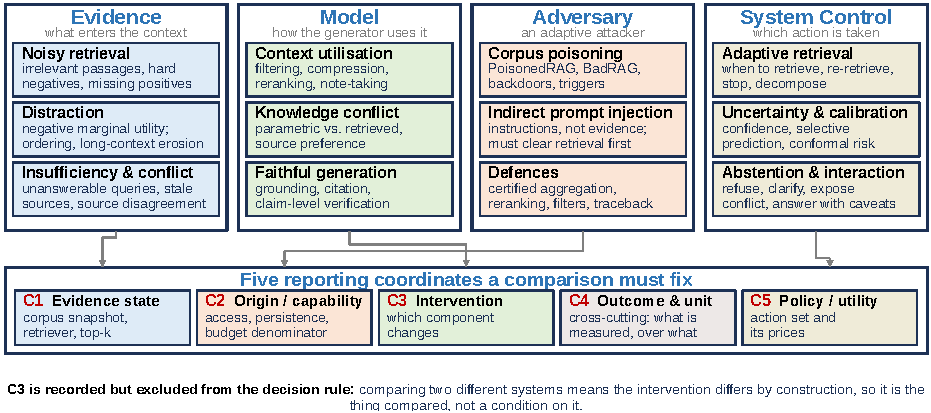
\includegraphics[width=\textwidth]{figures/generated/fig_taxonomy_map.pdf}%
\caption{The four failure surfaces and the reduction they support. Each column
is one surface of the survey (\S\ref{sec:evidence}--\S\ref{sec:system}); the
band below is the five reporting coordinates of \S\ref{sec:coordinates}, and the
connectors show which surface each coordinate collapses. C4 is cross-cutting
and has no single parent surface. The organisation is a partition of the
\emph{comparison} rather than of the literature: the columns tell a reader where
to look for related work, and the band tells a reader what must be stated on
both sides before two numbers can be placed together.}
\label{fig:hierarchical-taxonomy}
\end{figure*}


We model a RAG system as an evidence-conditioned decision process:
\[
q \rightarrow R(q, \mathcal{C}) \rightarrow E_q \rightarrow G(q, E_q, \theta) \rightarrow a \rightarrow y,
\]
where $q$ is a query, $\mathcal{C}$ is a corpus, $R$ is a retriever, $E_q$ is the retrieved evidence set, $G$ is the generator, $\theta$ denotes parametric model knowledge, $a$ is a system action, and $y$ is the final response. Robustness failures arise when $E_q$ is incomplete, irrelevant, misleading, conflicting, corrupted, or insufficient. The system must therefore both \emph{interpret evidence} and \emph{choose actions}.

Inspired by the perspective-based organization of recent ACL survey methodology, we organize robust RAG into four layers:
\begin{itemize}[leftmargin=*]
    \item \textbf{Evidence-centric robustness}: methods and failures concerning what enters the context, including noisy retrieval, hard negatives, distractors, and poisoned corpora.
    \item \textbf{Model-centric robustness}: methods and failures concerning how the generator uses evidence, including context filtering, faithfulness, attribution, and parametric--retrieved knowledge conflict.
    \item \textbf{System-centric control}: policies for when to retrieve, re-retrieve, verify, abstain, or ask for clarification under uncertainty and cost constraints.
    \item \textbf{Evaluation}: benchmarks and metrics that measure noise robustness, distraction sensitivity, conflict handling, attack success, calibration, selective risk, and action quality.
\end{itemize}

\begin{table*}[t]
\centering
\scriptsize
\renewcommand{\arraystretch}{0.88}
\begin{tabularx}{\linewidth}{>{\raggedright\arraybackslash}p{0.18\linewidth}>{\raggedright\arraybackslash}p{0.31\linewidth}>{\raggedright\arraybackslash}p{0.25\linewidth}X}
\toprule
\textbf{Boundary case} & \textbf{Rule used in this paper} & \textbf{Verdict consequence} & \textbf{Example implication} \\
\midrule
Noisy retrieval vs. distraction & Retrieval imperfection alone is coded as relevance/noise; harmful influence on generation, confidence, or reasoning is coded as distraction. & Same broad topic but different measured effect is partial. & Random negatives and hard distractors should not be pooled into one score. \\
Query/OOD vs. evidence state & Query ambiguity, distribution shift, and model uncertainty describe the need or belief state. Code them under origin unless the study labels the resulting retrieved evidence. & Shared uncertainty language does not imply a common evidence state or policy. & An OOD detector is not automatically an insufficient-context detector. \\
Natural conflict vs. adversarial corruption & Code by the source of contradiction, not by surface form. Naturally occurring or diagnostic contradiction is conflict; attacker-created contradiction is integrity/adversarial corruption. & Natural-conflict and poisoning results are invalid as a direct ranking unless the threat model is redefined. & Faithfulness or source-preference methods are not poisoning defenses by default. \\
Intervention mismatch & Code the component changed, then inspect the evaluation harness. Different interventions can be compared as alternatives if the remaining pipeline and target are controlled. & Shared harness and end-to-end target can support valid comparison; unmatched pipelines support only a qualified comparison. & A filter and a note-taking prompt can be compared after fixing retriever, generator, evidence states, budget, and action utility. \\
Metric overlap & Metric targets must match the object being measured. Accuracy, citation support, attack success, calibration, and selective risk are separate families. & Shared dataset but different metric family is partial; mutually incompatible targets are invalid for one-scalar ranking. & A correct answer with unsupported citation should not pass a faithfulness comparison. \\
Observable but unnamed action & Infer behavior only when action is decision-relevant and the protocol is unambiguous; otherwise use \emph{not applicable}. & Merely omitting the phrase ``action policy'' does not force under-specification. & An answer-only benchmark supplies \emph{answer} for a policy claim, but a fixed latency comparison needs no action label. \\
Security capability missing & Mark only decision-critical missing access, budget, objective, or target as unknown. A shared harness may intentionally vary capability. & Unknown capability makes a cross-game rank under-specified; controlled capability variation can support a valid descriptive contrast. & Black- and white-box variants of one attack can be compared inside the same harness without implying cross-paper transfer. \\
Benchmark vs. method & Code benchmark if the reusable artifact is the main contribution; otherwise code the intervention. & Benchmark-method comparison is partial unless the method is evaluated on the benchmark under aligned assumptions. & RGB is benchmark-first; RAAT is training-first. \\
Tuple match but control mismatch & After semantic coding, inspect corpus, data, retriever, generator, top-$k$, budget, baselines, decoding, and uncertainty. & A tuple match is insufficient for direct ranking when these factors confound the reported score. & Two answer-only noise methods on different datasets and generators require a shared rerun or a qualified claim. \\
\bottomrule
\end{tabularx}
\caption{Boundary rules for applying the revised diagnostic schema. Verdicts are claim-specific and require both semantic and experimental-control checks.}
\label{tab:taxonomy-rules}
\end{table*}


\paragraph{How Figure~\ref{fig:hierarchical-taxonomy} differs from Figure~\ref{fig:operational-pipeline-image}.}
Figure~\ref{fig:hierarchical-taxonomy} is a \emph{research landscape map}: it organizes the literature by where robustness problems and methods sit in the RAG stack. Its goal is taxonomic---to separate evidence-centric, model-centric, system-centric, and evaluation work. Figure~\ref{fig:operational-pipeline-image}, by contrast, is an \emph{operational system workflow}: it describes what a deployed robust RAG system should do when unreliable evidence is encountered. In short, Figure~\ref{fig:hierarchical-taxonomy} answers ``where does a paper fit?'', while Figure~\ref{fig:operational-pipeline-image} answers ``what should the system do next?''.

\begin{table*}[t]
\centering
\small
\begin{tabularx}{\linewidth}{p{0.14\linewidth}p{0.2\linewidth}p{0.27\linewidth}X}
\toprule
\textbf{Stage} & \textbf{Question} & \textbf{Typical signals} & \textbf{Representative actions} \\
\midrule
Detect & Is the current evidence unreliable? & Low retrieval confidence, high contradiction, low sufficient-context score, suspicious document patterns & Flag query/evidence, route to stronger checks, log risk state \\
Diagnose & What kind of unreliability is present? & Irrelevance, distraction, conflict, poisoning, ambiguity, unanswerability, stale evidence & Assign failure type; separate benign noise from adversarial risk \\
Mitigate & Can the evidence be repaired before answering? & Alternative retrieval results, filter scores, reranker utility, provenance, source agreement & Re-rank, filter, compress, re-query, retrieve from trusted sources, remove malicious passages \\
Control & What should the system do now? & Calibrated confidence, selective risk, cost budget, user risk tolerance & Answer, abstain, ask clarification, expose conflict, escalate to human review \\
Monitor & Did the system fail or get attacked? & User feedback, traceback signals, poisoned-document clusters, drift over time & Update index, quarantine sources, revise prompts, retrain filters, update audit logs \\
\bottomrule
\end{tabularx}
\caption{An operational pipeline for robust RAG. The pipeline turns the paper's taxonomy into actionable system design steps.}
\label{tab:operational-pipeline}
\end{table*}


\subsection{From Taxonomy to an Operational Pipeline}

A survey taxonomy is useful only if it helps researchers and practitioners decide what to build. We therefore translate the hierarchy into an operational pipeline: detect, diagnose, mitigate, control, and monitor (Table~\ref{tab:operational-pipeline}). This pipeline borrows the spirit of successful actionable surveys: first identify the object of intervention, then diagnose the mechanism, then apply a targeted intervention, and finally measure whether the intervention improves the desired system property.

\begin{figure*}[t]
\centering
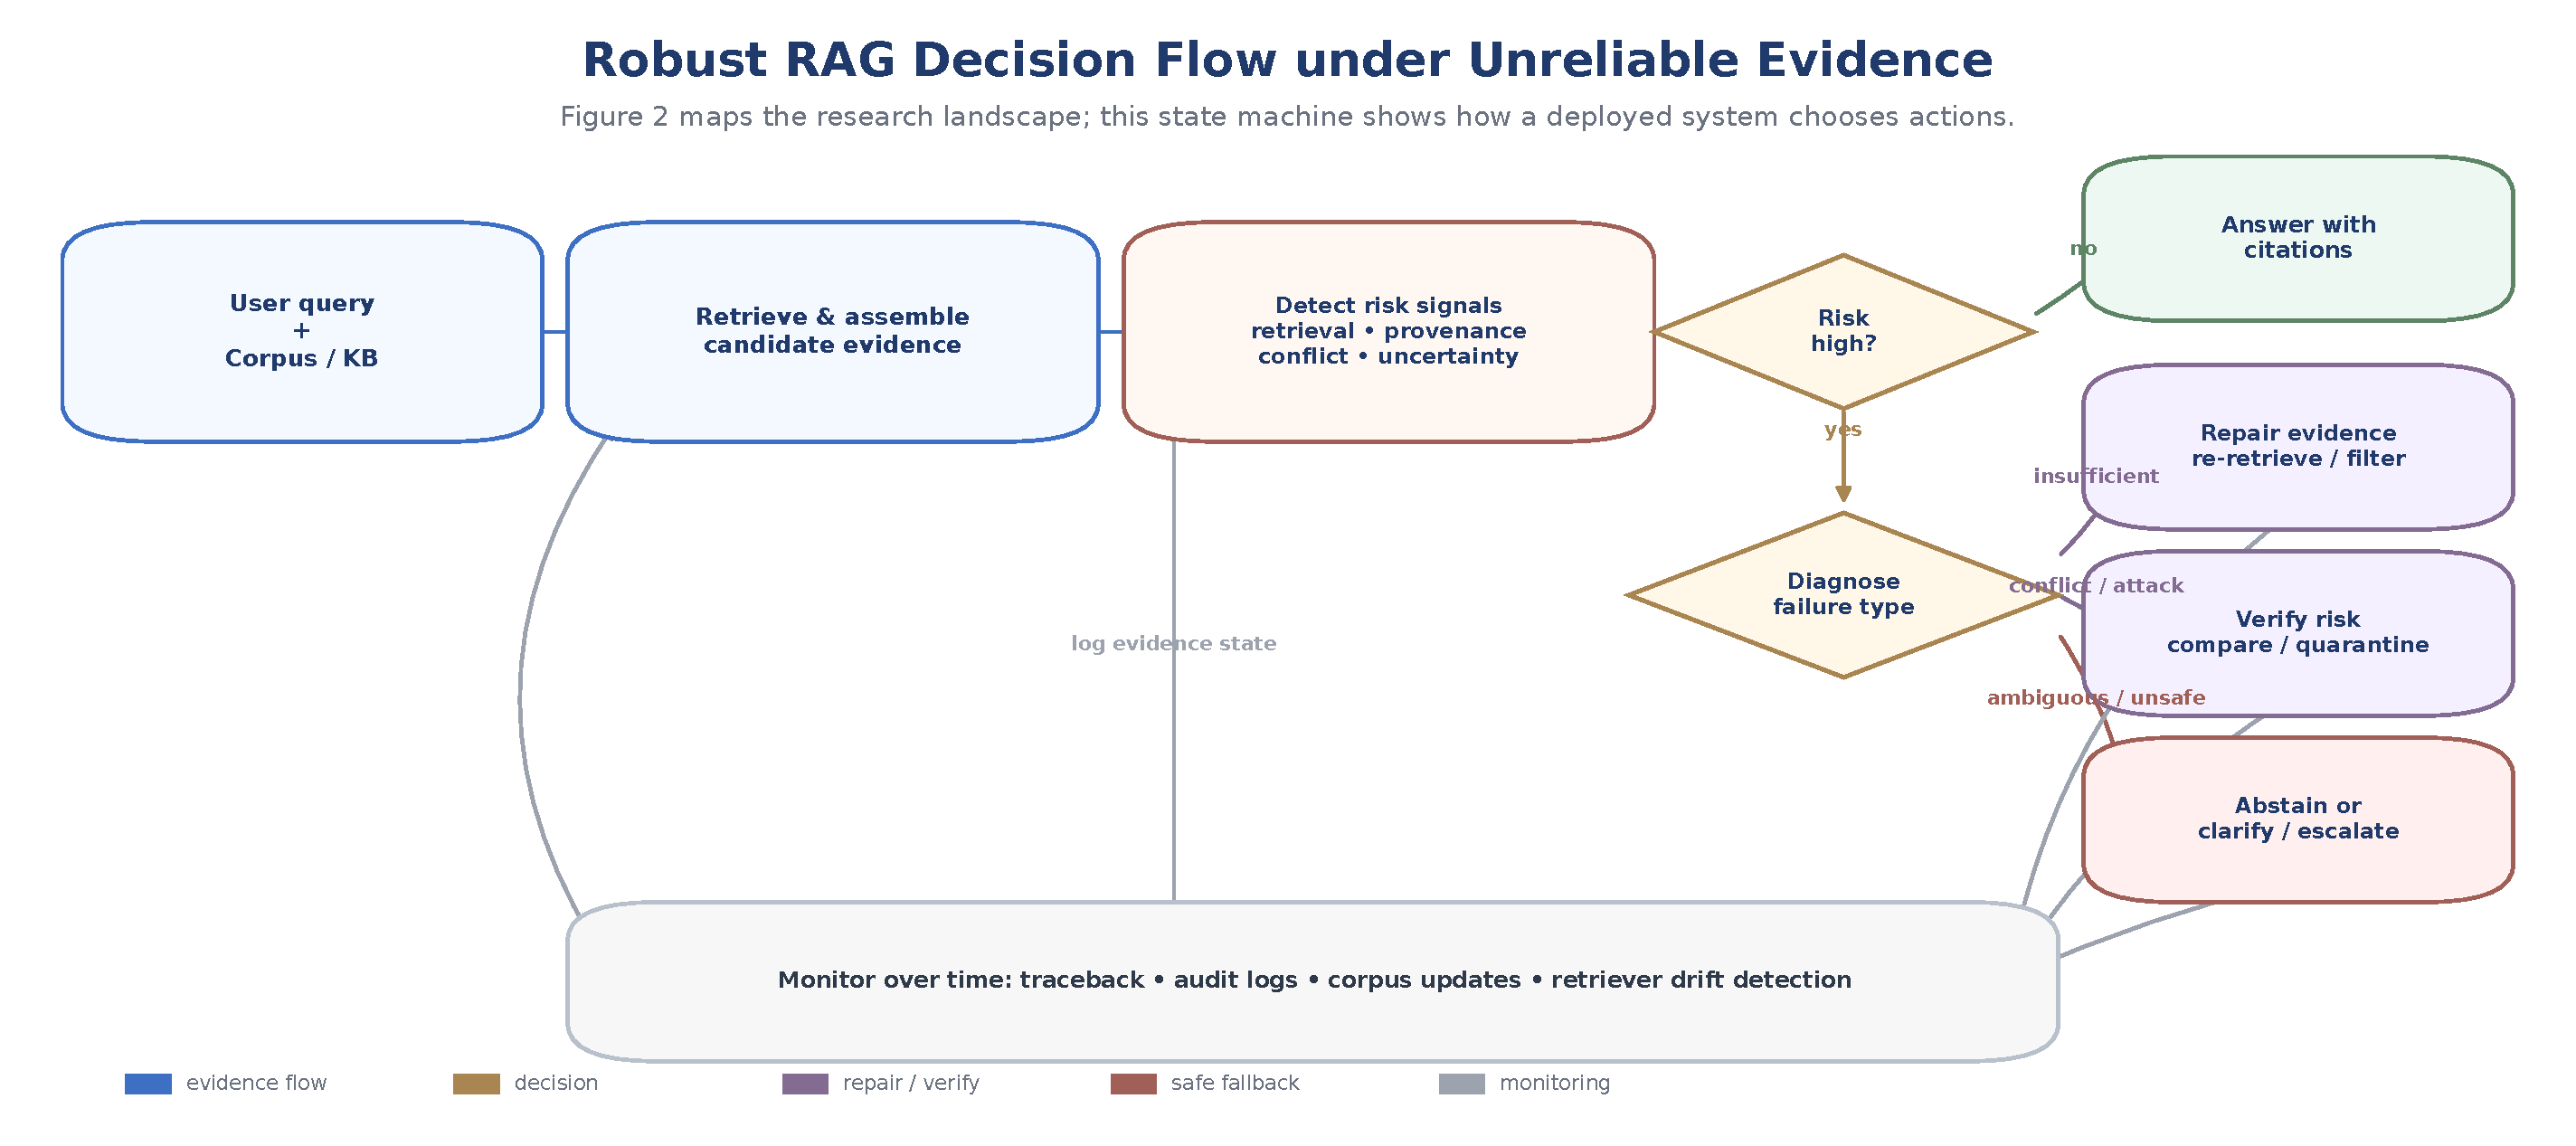
\includegraphics[width=\textwidth,keepaspectratio]{figures/generated/fig3_operational_decision_flow_py_4k.pdf}
\caption{Operational decision flow for robust RAG. Unlike the taxonomy in Figure~\ref{fig:hierarchical-taxonomy}, this state-machine view describes the branching actions a deployed system can take when unreliable evidence is encountered: answer, repair evidence, verify risk, abstain, clarify, escalate, or monitor.}
\label{fig:operational-pipeline-image}
\end{figure*}


\paragraph{Detect.}
Detection asks whether the current evidence state is risky. Signals can come from retrieval scores, disagreement among retrieved passages, low sufficient-context estimates, anomalous attention patterns, source provenance, or model uncertainty. Detection is intentionally broad: the system need not know the exact failure type yet. The goal is to decide whether the normal answer path is safe or whether stronger checks are needed.

\paragraph{Diagnose.}
Diagnosis assigns the likely failure mode. Is the context irrelevant, distracting, conflicting, poisoned, stale, ambiguous, or insufficient? This distinction is crucial because each failure requires a different response. Irrelevant context can be filtered; conflicting evidence may require source comparison; poisoned evidence may require quarantine or traceback; ambiguous queries may require clarification; insufficient context may require re-retrieval or abstention.

\paragraph{Mitigate.}
Mitigation attempts to repair the evidence state before generation. Evidence-centric mitigation includes reranking, filtering, context compression, retrieval diversification, and trusted-source retrieval. Model-centric mitigation includes note-taking, conflict-aware reasoning, fact-level alignment, and post-generation verification. Security mitigation includes document sanitization, poisoned-document detection, robust aggregation, and traceback. The best mitigation is failure-specific: a defense against prompt injection is not necessarily a defense against stale evidence.

\paragraph{Control and monitor.}
Control is the final decision: answer, abstain, ask a question, retrieve again, expose conflict, or escalate. Monitoring extends robustness beyond a single response. RAG corpora change over time; attacks may be discovered after release; user feedback can reveal missing evidence. Robust RAG therefore requires audit logs, source provenance, retriever drift monitoring, and mechanisms for removing or demoting harmful documents.

\begin{table*}[t]
\centering
\small
\begin{tabularx}{\linewidth}{p{0.15\linewidth}p{0.28\linewidth}p{0.28\linewidth}X}
\toprule
\textbf{Layer} & \textbf{Representative failures} & \textbf{Representative methods} & \textbf{Evaluation signals} \\
\midrule
Evidence-centric & Missing positives, irrelevant passages, hard negatives, poisoned documents & Retriever training, reranking, filtering, corpus sanitization, adversarial retrieval defenses & Recall under perturbation, poisoned retrieval rate, distractor sensitivity \\
Model-centric & Context over-reliance, parametric--retrieved conflict, unsupported generation & Context compression, note-taking, fact-level conflict modeling, source-aware reasoning, verification & Faithfulness, answer flips, conflict sensitivity, attribution quality \\
System-centric & Over-retrieval, under-retrieval, overconfidence, unanswerable queries & Adaptive retrieval, corrective retrieval, calibrated decision-making, selective generation, abstention & Selective risk, calibration error, retrieval-trigger accuracy, action cost \\
Evaluation & Fragmented benchmarks and non-comparable threat models & Stress tests, attack suites, uncertainty benchmarks, joint evaluation protocols & Robustness curves, attack success rate, defense bypass, action-quality metrics \\
\bottomrule
\end{tabularx}
\caption{The proposed hierarchy maps robust RAG from evidence failures to generator behavior, system control, and evaluation.}
\label{tab:hierarchy}
\end{table*}

\section{Evidence-Centric Robustness}
\label{sec:evidence}

Evidence-centric robustness concerns the quality, integrity, and sufficiency of the evidence that enters the context window. In classical information retrieval, irrelevant results are often treated as a ranking problem. In RAG, however, the retrieved set becomes part of the model input; a single misleading passage can change the generated answer, confidence, and citations. Evidence-centric work therefore asks three questions: what kinds of bad evidence appear, how do they affect generation, and which pre-generation controls can reduce their harm?

\begin{table*}[t]
\centering
\small
\begin{tabularx}{\linewidth}{p{0.18\linewidth}p{0.18\linewidth}p{0.25\linewidth}X}
\toprule
\textbf{Theme} & \textbf{Representative work} & \textbf{Core idea} & \textbf{What it reveals for robust RAG} \\
\midrule
Irrelevant context & \citetalias{irrelevantContext2023} & Analyze and mitigate irrelevant retrieved context with filtering and robust training & Even answerable questions degrade when irrelevant passages enter the context; robustness is not equivalent to retrieval recall. \\
Retrieval-noise training & \citetalias{raat2024} & Categorize retrieval noise and train with adaptive adversarial objectives & Noise types should be separated: irrelevant, relevant-but-insufficient, and counterfactual evidence have different effects. \\
Generator note-taking & \citetalias{chainOfNote2023} & Generate per-passage notes before answering & Robust generation benefits from intermediate relevance judgments rather than direct answer generation. \\
Fine-grained noise benchmark & \citetalias{rrag027} & Configurable benchmark for distracting, low-quality, inconsequential, and irrelevant noise & ``Noise'' is not monolithic; evaluation should vary type, amount, and placement of bad evidence. \\
Nonlinear distraction & \citetalias{rrag003} & Study disproportionate effect of small amounts of misleading information & A few strong distractors can dominate long-context reasoning, so average noise rate is insufficient. \\
Long-context RAG & \citetalias{rrag039} & Analyze long-input RAG and hard negatives & More retrieved context can hurt unless ordering, filtering, or training adapts to long-context failure modes. \\
Sentence-level filtering & \citetalias{rrag044} & Filter retrieved context before generation & Filtering can be more fine-grained than document reranking and can remove local distractors inside otherwise useful passages. \\
Retrieval evaluation & \citetalias{rrag058} & Utility-aware retrieval metric for LLMs & RAG retrieval should be evaluated by downstream utility, including negative utility from distracting passages. \\
\bottomrule
\end{tabularx}
\caption{Representative evidence-centric work on noisy retrieval and distraction.}
\label{tab:evidence-methods}
\end{table*}


\subsection{Retrieval Noise: Beyond Relevant vs. Irrelevant}

The earliest robust-RAG studies show that retrieval errors do not merely reduce recall; they alter the generator's behavior. \citet{irrelevantContext2023} demonstrate that retrieval-augmented language models can be brittle to irrelevant context and propose filtering and robust training as mitigation. This work is important because it separates two effects that are often conflated: a retriever may fail to retrieve enough relevant evidence, and a generator may fail to ignore irrelevant evidence once it is retrieved. Robustness therefore depends on both retriever quality and generator selectivity.

Subsequent work expands the typology of noise. \citet{raat2024} distinguishes multiple retrieval-noise types and trains models with adaptive adversarial objectives and explicit noise awareness. The distinction matters: an irrelevant passage that is obviously off-topic may be easy to ignore, while a counterfactual or hard-negative passage may be semantically close to the query and therefore much more dangerous. RGB similarly evaluates noise robustness, negative rejection, information integration, and counterfactual robustness as separate abilities \citep{rgb2023}. Taken together, these works suggest that ``RAG robustness'' cannot be measured by a single noisy-context accuracy number. A strong evaluation should vary the type, quantity, ranking position, and semantic hardness of negative evidence.

Recent benchmarks make this point more explicit. Magic Mushroom introduces fine-grained retrieval noise categories, including distracting and low-quality evidence \citep{rrag027}. URAG formulates uncertainty quantification in RAG and studies the effect of irrelevant and noisy retrieval on conformal prediction \citep{rrag001}. PRGB and other placeholder or perturbation-based benchmarks test whether models remain robust when retrieval context is systematically manipulated \citep{rrag183}. The trajectory of this literature is clear: robust RAG evaluation is moving from ``add random distractors'' to controlled stress tests that expose distinct failure mechanisms.

\subsection{Distraction and Context Utility}

Distraction is stronger than irrelevance. A passage is distracting when it has negative marginal utility: adding it changes the answer, confidence, attribution, or reasoning path in a harmful direction. This explains why more retrieval is not always better. In long-context settings, retrieving more passages can increase the chance that a hard negative appears before or near useful evidence. \citet{rrag039} study long-context RAG and show why ordering and hard negatives become central once the generator can consume many passages. \citet{rrag003} identify a nonlinear ``first drop of ink'' effect: a small amount of misleading information can disproportionately degrade reasoning. CUB evaluates context-utilization techniques across gold, conflicting, and irrelevant contexts \citep{rrag032}, while UDCG redefines retrieval evaluation around downstream utility rather than traditional relevance alone \citep{rrag058}.

This line of work changes the role of the retriever. The retriever is not only a recall engine; it is a context constructor. A retriever optimized for lexical or embedding similarity may return passages that are highly related to the query but harmful to the generator. A robust retriever should consider downstream answer utility, redundancy, conflict, and the interaction between passages. Similarly, a robust RAG system should not treat the top-$k$ list as a fixed input. It should be able to filter, reorder, compress, diversify, or abstain when the context set is unreliable.

\subsection{Evidence-Side Mitigations}

Evidence-side defenses operate before or during context construction. They include retriever retraining, reranking, filtering, passage compression, and context ordering. Filtering can be document-level or sentence-level. FILCO-style sentence filtering removes irrelevant local content inside otherwise useful passages \citep{rrag044}; this is important because a retrieved document can contain both answer evidence and distracting details. Utility-aware retrieval metrics and rerankers attempt to optimize what helps the generator, not what merely matches the query \citep{rrag058}. Context ordering and long-context tuning address cases where the same evidence set has different effects depending on position \citep{rrag039}.

Training-based approaches expose the generator to noise so that it learns to separate relevant from irrelevant context \citep{raat2024,rrag091}. This can improve robustness but also raises a scalability question: robust training may be less effective or less necessary as base LLMs become stronger, and adversarially generated noise can overfit to a particular retriever or generator. Training-free approaches, such as filtering and note-taking, are easier to add to existing systems but depend on reliable relevance or sufficiency signals. A recurring pattern is that no single pre-generation control is sufficient: retrieval filtering reduces easy noise, reranking handles ordering, compression improves context budget, and downstream calibration remains necessary for residual uncertainty.

\subsection{Query-Side and Index-Side Sources of Noise}

Evidence noise does not begin at retrieval scoring. Query formulation is itself a brittle interface. Query-level robustness work shows that minor changes in wording can substantially affect retrieval and downstream answers \citep{queryRobustness2025}. This suggests that robust RAG should include query normalization, query expansion, and query uncertainty estimation. In multi-turn settings, the query may be non-standalone or under-specified, making retrieval quality depend on dialogue state tracking \citep{rrag141}. The retriever may also inherit biases from chunking and indexing: relevant facts can be split across chunks, qualifiers can be separated from claims, and embeddings can overemphasize topical similarity over answer sufficiency.

Index-side design also changes robustness. Smaller chunks improve retrieval granularity but can remove context needed for factual interpretation. Larger chunks preserve context but increase the chance of including distracting material. Hybrid sparse--dense retrieval can reduce some embedding failures but may increase redundancy. Graph-based, multimodal, and agentic/process-level RAG add structure but introduce new poisoning surfaces, as shown by GraphRAG poisoning, graph poisoning, and reasoning-style poisoning work \citep{rrag051,rrag127,rrag175}. Thus, evidence-centric robustness should be studied as a corpus construction problem, not only as a retriever ranking problem.

\subsection{Design Tradeoffs}

Evidence-side controls have three recurring tradeoffs. First, filtering improves precision but can remove weakly relevant evidence needed for multi-hop reasoning. Second, reranking can demote distractors but may also amplify model-specific biases if the reranker is trained against a narrow generator. Third, context compression saves tokens but can delete qualifiers, source information, or uncertainty markers. Robust RAG systems should therefore expose confidence about filtering decisions and allow later stages to recover from false negatives. A practical design is multi-stage: retrieve broadly, rerank cautiously, filter locally, preserve provenance, and let the generator or verifier request more evidence when sufficiency is low.

\section{Model-Centric Robustness}
\label{sec:model}

Model-centric robustness concerns how the generator interprets, weighs, and integrates evidence once it appears in the prompt. Even with the same retrieved context, different generators can answer differently because they vary in instruction following, parametric prior strength, context utilization, and calibration. Model-centric work therefore studies the internal and behavioral mechanisms that determine whether retrieved evidence is used faithfully or misleadingly.

\begin{table*}[t]
\centering
\small
\begin{tabularx}{\linewidth}{p{0.2\linewidth}p{0.2\linewidth}p{0.28\linewidth}X}
\toprule
\textbf{Problem} & \textbf{Representative work} & \textbf{Mechanism} & \textbf{Limitation or open issue} \\
\midrule
Parametric--retrieved conflict & \citetalias{tugOfWar2024} & Construct and analyze conflicts between internal and external knowledge & Conflict behavior depends on model, prompt, evidence coherence, and task framing. \\
Fact-level conflict modeling & \citetalias{faithfulRAG2025} & Extract parametric self-facts, align them with retrieved facts, and reason before answering & Requires reliable fact extraction and alignment; complex claims remain difficult. \\
Source-aware consolidation & \citetalias{astuteRAG2025} & Elicit internal knowledge and consolidate it with retrieved sources using reliability comparison & Training-free but still depends on LLM self-assessment and source-quality cues. \\
Hidden-state rectification & \citetalias{rrag008} & Locate layers where parametric suppression occurs and contrast contextual/non-contextual logits & Promising for model-centric control, but model internals and transferability remain open. \\
Context utilisation benchmarks & \citetalias{rrag032} & Test gold, conflicting, and irrelevant contexts across models & Benchmarks reveal whether a model uses context, but not always why a model chooses one source. \\
Real-document conflict & \citetalias{rrag112} & Study behavior under context-memory conflicts with real documents & Realistic evidence can be messier than synthetic conflicts and harder to label. \\
Source preference & \citetalias{rrag132} & Analyze which sources win under conflict & Source preference may encode bias, recency effects, or authority priors. \\
\bottomrule
\end{tabularx}
\caption{Representative model-centric work on knowledge conflict and contextual faithfulness.}
\label{tab:conflict-methods}
\end{table*}


\subsection{Context Utilization and Intermediate Reasoning}

One model-centric strategy is to force the generator to process evidence more explicitly before answering. Chain-of-Note asks the model to write notes for each retrieved passage, assess relevance, and abstain when evidence is insufficient \citep{chainOfNote2023}. This moves the generator from direct answer synthesis to a read--judge--answer pipeline. The value of this design is not simply better prompting; it externalizes intermediate evidence judgments that can be inspected, scored, or used to trigger abstention.

Other approaches manipulate the context itself. Context compression and filtering reduce the amount of irrelevant information passed to the model, while context-utilization benchmarks test whether models actually rely on gold evidence when it is present and ignore conflicting or irrelevant evidence when it is not \citep{rrag032}. The key distinction is between \emph{context availability} and \emph{context use}. A passage can be present in the prompt but ignored; a misleading passage can be unsupported but still dominate the answer. Thus, robust RAG must evaluate how models allocate attention, probability mass, and rationales across sources.

\subsection{Parametric--Retrieved Knowledge Conflict}

RAG introduces a conflict structure that does not exist in standard closed-book generation. The model has parametric memory, the retriever supplies external evidence, and multiple retrieved passages may disagree. When these sources conflict, models can exhibit two opposite failures: over-compliance with false retrieved evidence or stubborn reliance on stale parametric knowledge. Tug-of-War constructs and studies internal--external conflict in retrieval-augmented language models \citep{tugOfWar2024}. Adaptive Chameleon and related work show that LLMs can be highly receptive to coherent counter-evidence but resistant under other conflict conditions \citep{rrag046}. Real-document conflict studies show that behavior under conflict is not only a synthetic benchmark artifact \citep{rrag112}.

Conflict-aware methods differ in granularity. FaithfulRAG extracts parametric self-facts, aligns them with retrieved facts, localizes discrepancies, and uses a self-thinking step before generation \citep{faithfulRAG2025}. CoRect applies hidden-state and logit rectification to resolve conflicts without full model retraining \citep{rrag008}. Astute RAG elicits internal knowledge and consolidates it with retrieved passages through source-aware reliability comparison \citep{astuteRAG2025}. These methods share a principle: conflict should be represented explicitly before the final answer is produced.

\subsection{From Faithfulness to Source Reliability}

Many faithful RAG methods implicitly assume that retrieved context should be trusted. Robust RAG cannot make this assumption. Retrieved context can be stale, poisoned, incomplete, or irrelevant; parametric knowledge can be outdated or hallucinated. The correct policy depends on source reliability. Source preference studies ask which sources win under conflict \citep{rrag132}; ``who's who'' style evaluations study behavior under practical entity-level conflicts \citep{rrag110}. These works suggest that future systems should represent not only claims but also provenance, timestamp, authority, and consistency. In a high-stakes setting, the most robust answer may not be a single synthesized fact; it may be a statement that exposes disagreement and explains why one source is more credible.

\subsection{Citation, Attribution, and Verification}

RAG systems are often expected to cite sources, but citations do not guarantee faithfulness. A model can cite a passage that is topically related but does not support the generated claim, or cite the correct document while generating a claim from parametric memory. RAGTruth provides fine-grained hallucination annotations for RAG outputs \citep{ragTruth2024}. Related grounding methods train models to quote source spans or decompose external and parametric semantics, but these are not substitutes for claim-level citation verification \citep{rrag115,rrag206}. The key challenge is granularity. Document-level citation is too coarse when a passage contains multiple claims, qualifiers, or contradictions. Claim-level or sentence-level attribution is more informative but requires reliable entailment, alignment, and segmentation.

Verification can be pre-generation, post-generation, or iterative. Pre-generation verification asks whether the context is sufficient and trustworthy before answering. Post-generation verification checks whether each generated claim is supported by the evidence. Iterative verification alternates between generation and retrieval, using detected gaps or conflicts to form new queries. The limitation is cost: verification often requires additional model calls, retrieval calls, or entailment models. Robust RAG therefore needs cheap first-pass signals for routine cases and stronger verification for high-risk cases.

\subsection{Limits of Model-Centric Fixes}

Model-centric methods can improve evidence use, but they cannot fully solve evidence unreliability. A generator cannot reliably infer provenance if the corpus does not preserve it. It cannot resolve a conflict if all sources are equally stale or poisoned. It cannot calibrate answerability if retrieval never exposes missing evidence. Conversely, evidence-side controls cannot guarantee faithful generation. This complementarity motivates the layered framework: evidence-centric controls shape the input distribution, model-centric controls shape context use, and system-centric controls decide when the remaining uncertainty is too high to answer.

\section{Adversarial Corruption and Security}
\label{sec:adversarial}

Adversarial corruption is evidence unreliability under an adaptive attacker. RAG systems are vulnerable because they externalize memory into corpora, indices, prompts, and tools. An attacker can target any of these surfaces: the corpus before indexing, the retriever during matching, the prompt template, the retrieved context, or the downstream agent that executes actions.

\begin{table*}[t]
\centering
\small
\begin{tabularx}{\linewidth}{p{0.17\linewidth}p{0.19\linewidth}p{0.25\linewidth}X}
\toprule
\textbf{Attack/defense surface} & \textbf{Representative work} & \textbf{Threat or defense} & \textbf{Implication} \\
\midrule
Retriever poisoning & \citetalias{poisoningRetrievalCorpora2023} & Inject adversarial passages to manipulate dense retrievers & Retrieval security can fail before generation begins. \\
RAG knowledge corruption & \citetalias{poisonedRAG2024} & Craft malicious passages that steer generated answers & End-to-end RAG needs corpus integrity and generation safeguards. \\
Backdoor attacks & \citetalias{trojanRAG2024}; \citetalias{phantom2024} & Triggered retrieval/generation behavior via poisoned contexts & RAG can act as a backdoor carrier without modifying model weights. \\
Prompt template attacks & \citetalias{aip2025} & Weaponize shared instructional prompts to steer retrieval and generation & Prompt templates are part of the attack surface, not just implementation details. \\
Indirect prompt injection & \citetalias{rrag005} & Optimize trigger fragments so malicious instructions are retrieved in the wild & Real attacks must overcome the retrieval barrier, not merely place malicious text in a corpus. \\
Certified defense & \citetalias{certifiedRAG2024} & Isolate-and-aggregate answers for robustness certificates & Certification gives stronger guarantees but typically assumes specific attack budgets. \\
Reranking defense & \citetalias{rrag004} & Use probe-gradient instability to demote poisoned passages & Defense can be inserted retriever-side without retraining the LLM. \\
Attention defense & \citetalias{rrag015} & Detect poisoning via normalised attention variance & Internal attention signals may expose poisoned evidence, but adaptivity remains a concern. \\
\bottomrule
\end{tabularx}
\caption{Representative adversarial corruption attacks and defenses.}
\label{tab:adversarial-methods}
\end{table*}

\begin{table*}[t]
\centering
\scriptsize
\renewcommand{\arraystretch}{0.88}
\begin{tabularx}{\linewidth}{>{\raggedright\arraybackslash}p{0.18\linewidth}c c c c >{\raggedright\arraybackslash}p{0.15\linewidth}X}
\toprule
\textbf{Threat class} & \textbf{Corpus} & \textbf{Query} & \textbf{Retr.} & \textbf{Gen.} & \textbf{Objective} & \textbf{Boundary} \\
\midrule
Dense-retriever poisoning \citep{poisoningRetrievalCorpora2023} & write & train set & white/gray & no & retrieve bad passages & Not always end-to-end. \\
RAG knowledge corruption \citep{poisonedRAG2024,badRAG2024} & write & target topic & black/gray & black & answer steering & Stealth/dynamics vary. \\
Backdoor-style RAG \citep{trojanRAG2024,phantom2024} & write & trigger & gray & black & latent behavior & Normal queries may pass. \\
Indirect prompt injection \citep{aip2025,rrag005} & write/share & natural & black & black & instruction hijack & Must overcome retrieval. \\
Opinion/fairness manipulation \citep{rrag104,rrag162} & write & group/topic & black/gray & black & bias steering & QA metrics miss social harm. \\
Defense setting \citep{certifiedRAG2024,rrag004,rrag015,rrag128} & bounded & varies & assumed & black/gray & detect/demote/trace & Depends on budget/visibility. \\
\bottomrule
\end{tabularx}
\caption{Attacker-capability matrix for adversarial RAG. The same ``attack success rate'' can mean different things depending on corpus write access, query control, retriever visibility, generator access, and objective.}
\label{tab:attacker-capability}
\end{table*}

\begin{table*}[t]
\centering
\scriptsize
\renewcommand{\arraystretch}{0.88}
\begin{tabularx}{\linewidth}{>{\raggedright\arraybackslash}p{0.17\linewidth}>{\raggedright\arraybackslash}p{0.21\linewidth}>{\raggedright\arraybackslash}p{0.22\linewidth}>{\raggedright\arraybackslash}p{0.16\linewidth}X}
\toprule
\textbf{Comparison} & \textbf{Why it looks comparable} & \textbf{Hidden mismatch} & \textbf{Metric pitfall} & \textbf{Normalised reading} \\
\midrule
PoisonedRAG vs. dense-retriever poisoning & Both insert malicious evidence into a retrieval corpus. & One evaluates end-to-end answer steering; the other may evaluate retriever ranking before generation. & Retrieval success and answer attack success are not the same target. & Compare only after recording whether poisoned evidence is retrieved and whether the generator changes the final answer. \\
Certified RAG defense vs. prompt-injection defense & Both are RAG defenses against corrupted retrieved content. & Certification assumes a bounded number of corrupted passages; prompt injection exploits instruction following rather than only false facts. & A certificate under bounded corruption may not imply instruction-hijack resistance. & Treat certification, instruction isolation, and document sanitisation as complementary defenses. \\
Traceback vs. prevention & Both reduce harm after poisoning. & Traceback identifies influential poisoned documents after failure; prevention attempts to block harmful output before response. & Lower post-hoc traceback error does not equal lower user-facing attack success. & Report prevention, detection, demotion, traceback, and recovery as separate outcome variables. \\
Backdoor trigger vs. natural query attack & Both can produce targeted malicious behavior. & Trigger attacks may rely on rare phrases; natural-query attacks must survive ordinary retrieval and ranking. & Attack success under attacker-crafted triggers overstates risk under natural user queries. & Require query-control and trigger-frequency fields before comparing attack strength. \\
\bottomrule
\end{tabularx}
\caption{Concrete examples of threat-model normalisation. These cases show how reported attack or defense success can reverse when attacker access, retrieval realism, and evaluation target differ.}
\label{tab:threat-model-examples}
\end{table*}



\subsection{Corpus and Retriever Poisoning}

Corpus poisoning attacks insert malicious passages into the retrieval database so that they are returned for target queries. Early work on poisoning retrieval corpora demonstrates that small numbers of adversarial passages can manipulate dense retrieval \citep{poisoningRetrievalCorpora2023}. PoisonedRAG extends this threat to end-to-end generation: retrieved malicious passages can cause the LLM to output attacker-chosen answers \citep{poisonedRAG2024}. BadRAG, UniC-RAG, and related methods explore different trigger structures, optimization objectives, and attack settings \citep{badRAG2024,rrag049,rrag057}. The important lesson is that retrieval augmentation can amplify small corpus changes into large generation effects.

Backdoor-style attacks make the threat more persistent. TrojanRAG and Phantom show that triggers can activate malicious behavior through retrieved contexts without changing the generator weights \citep{trojanRAG2024,phantom2024}. Other attacks optimize token-level substitutions, influential tokens, or attention-steering patterns \citep{rrag050,rrag052,rrag120}. These works expose a system risk: a RAG system may appear safe under normal queries but fail under targeted concepts, phrases, or document manipulations.

\subsection{Indirect Prompt Injection and Prompt-Level Attacks}

Indirect prompt injection differs from factual poisoning. Instead of inserting false evidence, the attacker inserts instructions that are retrieved and interpreted by the LLM as commands. In practice, an indirect prompt injection must overcome the retrieval barrier: the malicious document must actually be retrieved under natural queries. \citet{rrag005} explicitly study this barrier and propose trigger fragments that improve retrieval of attack fragments. AIP broadens the surface further by showing that shared instructional prompts can be weaponized to steer RAG retrieval and generation \citep{aip2025}. These attacks imply that prompt templates, document ingestion rules, and retrieved text should be treated as untrusted inputs.

\subsection{Defenses and Their Assumptions}

Defenses against adversarial corruption operate at multiple layers. Certified approaches such as RobustRAG isolate and aggregate outputs to provide guarantees under bounded retrieval corruption \citep{certifiedRAG2024}. Reranking defenses such as ProGRank use instability or probe-gradient signals to demote suspicious passages \citep{rrag004}. Attention-based filters detect abnormal attention patterns caused by poisoned evidence \citep{rrag015}. Clustering and conflict-resolution defenses such as TrustRAG and SeCon-RAG filter semantically inconsistent or suspicious evidence before generation \citep{rrag013,rrag017}. Traceback methods attempt to identify poisoned texts after an attack has occurred \citep{rrag128}.

The main limitation is threat-model fragmentation. A defense designed for corpus poisoning may not stop prompt-template attacks; a filter trained on obvious malicious instructions may not detect fact-level poisoning; a certified aggregation method may assume a corruption budget that is hard to estimate in open corpora. Robust RAG security therefore needs compositional evaluation: combine poisoned facts, retrieval triggers, prompt-bearing documents, and benign noise in the same pipeline.

\subsection{Threat Model Dimensions}

Security papers differ in attacker knowledge, access, and objective. Some assume the attacker can insert a few documents into a public corpus but cannot see user queries. Others assume black-box query access, white-box retriever gradients, control over prompt templates, or access to agent memory. Objectives also differ: targeted answer steering, denial of service, refusal induction, opinion manipulation, privacy extraction, fairness manipulation, or guardrail bypass. Comparing attacks without specifying these dimensions is misleading. A poisoning method that works with five injected documents under black-box access has stronger practical relevance than a method requiring full index control; a defense evaluated only against keyword triggers may fail against semantic triggers.

Table~\ref{tab:attacker-capability} makes this comparison explicit. We separate corpus write access, query control, retriever visibility, generator access, and objective because they determine whether two attack results are comparable. This matrix also clarifies why benign retrieval noise and adversarial corruption should not be collapsed into a single robustness score: the former tests system tolerance to accidental evidence errors, while the latter tests adaptive pressure against the retrieval-generation interface.

\subsection{Attack Success Is Not Enough}

Attack success rate is necessary but insufficient. A strong RAG attack must also be stealthy, durable, and retrieval-realistic. Stealth means poisoned passages should not be trivially detected by lexical filters or human inspection. Durability means attacks should persist under chunking, reranking, context filtering, and prompt changes. Retrieval realism means the malicious content must be retrieved under natural user queries, not only under attacker-crafted queries. Work on indirect prompt injection in the wild explicitly highlights this retrieval barrier \citep{rrag005}. Recent stealth and attention-aware work similarly argues that defenses should evaluate whether poisoned content can be distinguished from benign evidence \citep{rrag015}.

\subsection{Defense-in-Depth}

The surveyed defenses suggest a defense-in-depth architecture. At ingestion time, systems should validate sources, scan documents for prompt-like instructions, preserve provenance, and detect anomalous clusters. At retrieval time, systems can rerank with robustness signals, compare retrieved documents for contradictions, and demote passages with suspicious trigger behavior. At generation time, systems should isolate evidence from instructions, verify answer support, and refuse to execute instructions found in retrieved documents. During operation, systems need logging and traceback to identify which corpus items influenced harmful outputs. No layer is sufficient alone, but layered controls reduce the chance that one bypass compromises the entire pipeline.

\section{System-Centric Control}
\label{sec:control}

System-centric control treats RAG as a policy rather than a fixed pipeline. A robust system must decide whether to retrieve, how much to retrieve, whether to re-retrieve, whether to verify, whether to trust internal knowledge, and whether to answer at all. This layer is where evidence reliability becomes an action.

\begin{table*}[t]
\centering
\small
\begin{tabularx}{\linewidth}{p{0.16\linewidth}p{0.18\linewidth}p{0.28\linewidth}X}
\toprule
\textbf{Control/evaluation question} & \textbf{Representative work} & \textbf{Signal or decision} & \textbf{Why it matters} \\
\midrule
When to retrieve & \citetalias{selfRAG2023}; \citetalias{whenToRetrieve2024}; \citetalias{ctrla2025} & Reflection tokens, special retrieval tokens, or representation-based confidence/honesty directions & Retrieval is an action with costs and risks, not a fixed preprocessing step. \\
When retrieval is weak & \citetalias{crag2024}; \citetalias{sufficientContext2024} & Retrieval evaluator or sufficient-context signal & A system should repair or abstain rather than answer from insufficient evidence. \\
Calibration & \citetalias{calibRAG2025}; \citetalias{uncertaintyRAG2024}; \citetalias{rrag007} & Decision calibration, span uncertainty, verbal confidence calibration & Robustness requires confidence to reflect both model and evidence uncertainty. \\
Unanswerability & \citetalias{rrag111}; \citetalias{rrag141} & Unanswerable and underspecified RAG benchmarks & Real users often ask questions the corpus cannot answer; refusal and clarification need direct evaluation. \\
RAG capabilities & \citetalias{rgb2023} & Noise robustness, negative rejection, integration, counterfactual robustness & Multi-axis evaluation exposes failures hidden by answer accuracy. \\
Hallucination detection & \citetalias{ragTruth2024} & Word-level hallucination annotations for RAG outputs & Fine-grained labels support detection and attribution beyond answer-level scoring. \\
Query robustness & \citetalias{queryRobustness2025} & Perturb query wording and measure pipeline sensitivity & Robustness must include the query-to-retrieval interface. \\
\bottomrule
\end{tabularx}
\caption{Representative work on system-centric control and evaluation.}
\label{tab:control-eval-methods}
\end{table*}

\begin{table*}[t]
\centering
\scriptsize
\renewcommand{\arraystretch}{0.9}
\begin{tabularx}{\linewidth}{>{\raggedright\arraybackslash}p{0.18\linewidth}>{\raggedright\arraybackslash}p{0.22\linewidth}>{\raggedright\arraybackslash}p{0.25\linewidth}X}
\toprule
\textbf{Lineage} & \textbf{Classical question} & \textbf{RAG-specific version} & \textbf{Why it matters for robust RAG} \\
\midrule
Selective prediction & When should a model abstain to control risk? & Abstain when retrieved evidence is insufficient, conflicting, stale, or corrupted. & Selective risk must condition on evidence state, not only answer confidence. \\
Calibration & Does confidence match correctness? & Does confidence match answer correctness, evidence sufficiency, citation support, and retrieval usefulness? & A calibrated answer probability can still hide unreliable evidence. \\
Active clarification & When should the system ask a user for more information? & Ask clarification before retrieval when the query is ambiguous or underspecified. & Clarification can be the correct action even when retrieval could produce a plausible answer. \\
Cost-sensitive retrieval & When is additional computation worth it? & Decide whether to retrieve, re-retrieve, verify, rerank, or escalate under latency/cost budgets. & Robustness gains should be reported with action cost and coverage, not only accuracy. \\
Decision-theoretic control & Which action minimizes expected risk? & Choose among answer, abstain, expose conflict, cite uncertainty, retrieve again, or quarantine evidence. & Action quality is the bridge between evidence reliability estimates and user-facing behavior. \\
\bottomrule
\end{tabularx}
\caption{Action-control lineage. The framework imports ideas from selective prediction, calibration, clarification, and cost-sensitive decision-making, but makes retrieved evidence state the object being controlled.}
\label{tab:action-control-lineage}
\end{table*}



\subsection{Answerability and Sufficient Context}

The most basic control question is whether the available evidence is sufficient. RGB's negative rejection task and counterfactual robustness task show that RAG systems often answer when they should reject unsupported or false evidence \citep{rgb2023}. Sufficient Context reframes the problem: rather than asking whether the model can answer, ask whether the retrieved context contains enough information to answer \citep{sufficientContext2024}. Unanswerability benchmarks extend this idea to underspecified and unsupported queries \citep{rrag111,rrag141}.

This line of work separates two forms of uncertainty. \emph{Evidence uncertainty} asks whether the corpus and retrieved context support the answer. \emph{Model uncertainty} asks whether the generator can integrate the evidence correctly. A system can have high model confidence but low evidence sufficiency, which is dangerous. Conversely, a system may have adequate evidence but low model confidence, suggesting verification or decomposition rather than refusal.

\subsection{Adaptive Retrieval and Retrieval Budgets}

Always retrieving is inefficient and can be harmful; never retrieving leaves the model dependent on stale parametric knowledge. Adaptive retrieval methods learn or infer when external evidence is needed. Self-RAG trains models to retrieve, generate, and critique with reflection tokens \citep{selfRAG2023}. Adapt-LLM-style methods use explicit retrieval tokens to signal when retrieval is needed \citep{whenToRetrieve2024}. CtrlA uses representation-level honesty and confidence directions to guide retrieval timing \citep{ctrla2025}. Corrective RAG uses a retrieval evaluator to trigger additional retrieval or web search when the initial evidence is weak \citep{crag2024}.

Recent work also shows that retrieval can be over-used. Over-searching studies introduce metrics such as tokens-per-correctness and benchmarks that measure when search-augmented systems retrieve unnecessarily \citep{rrag006}. Adaptive retrieval without self-knowledge benchmarks many uncertainty-estimation methods and shows that retrieval policies must be evaluated for both accuracy and efficiency \citep{rrag034}. The emerging view is that retrieval is a budgeted decision: each retrieval step trades cost, latency, exposure to noise, and potential accuracy gain.

\subsection{Calibration, Abstention, and Interaction}

Calibration asks whether confidence matches correctness. In RAG, confidence depends on both model uncertainty and evidence uncertainty. CalibRAG optimizes for calibrated decision-making \citep{calibRAG2025}; UncertaintyRAG uses span-level uncertainty to improve retrieval training and robustness under distribution shift \citep{uncertaintyRAG2024}; noise-aware verbal confidence calibration targets overconfidence under irrelevant or counterfactual retrieval \citep{rrag007}. SABER-style trust-or-abstain approaches estimate whether parametric knowledge and contextual knowledge paths are reliable, then map them to trust and abstention decisions \citep{rrag002}.

Abstention should not be treated as a single fallback string. A RAG system can refuse, ask a clarifying question, retrieve more, answer partially with caveats, or expose conflicting evidence. Multi-turn unanswerability benchmarks show that robust systems must distinguish between genuinely unanswerable questions, underspecified questions requiring clarification, and answerable questions requiring retrieval \citep{rrag141}. The next step is interactive calibration: a system should not only know when it is uncertain but also choose the user-facing action that best reduces risk.

\subsection{Policy Composition}

Most control methods study one decision at a time: retrieve or not, abstain or answer, verify or skip. Deployed RAG systems need policy composition. For example, if a query is ambiguous, the system should ask clarification before retrieval; if retrieval is low-confidence, it should re-query or broaden the corpus; if evidence conflicts, it should verify sources and expose disagreement; if a document contains instructions, it should treat them as data rather than commands. These actions have dependencies. Abstention after one weak retrieval may be premature if re-retrieval is cheap; re-retrieval after detecting poisoning may be unsafe if the corpus itself is compromised. A full control policy should represent state: query ambiguity, retrieval confidence, evidence sufficiency, conflict level, adversarial risk, and user risk tolerance.

\subsection{Cost, Latency, and Deployment Constraints}

Control policies are constrained by cost and latency. Multi-query retrieval, reranking, entailment verification, and self-consistency can improve reliability but increase token cost and response time. Over-searching work makes this explicit by measuring the cost of unnecessary search \citep{rrag006}. In organizational settings, retrieval may also be constrained by access control, privacy, and logging requirements. A useful research direction is risk-adaptive computation: cheap pipelines for low-risk queries, stronger verification for high-risk domains, and human review for cases with high uncertainty or high potential harm.

\section{Evaluation}
\label{sec:evaluation}

% Drawn by scripts/revision3/fig_appendix_schematics.py; the .pptx is the
% editable source and is released with the paper.
\begin{figure*}[t]
\centering
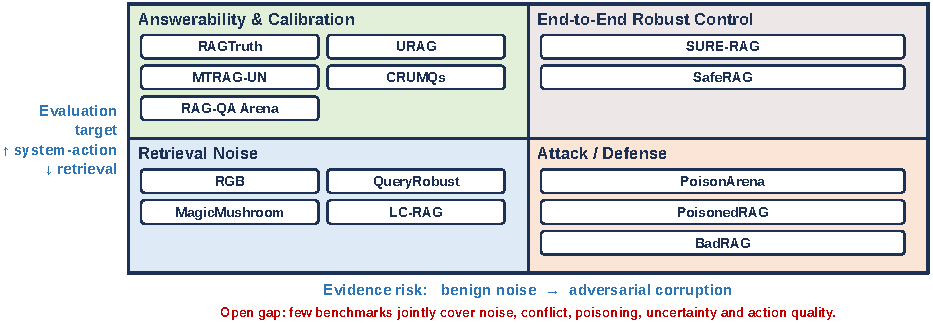
\includegraphics[width=\textwidth]{figures/generated/fig_benchmark_landscape.pdf}%
\caption{Conceptual benchmark landscape. Placement is illustrative rather than
data-derived; the figure organises differences in evidence risk and evaluation
level, not empirical distance or benchmark quality. The two axes are
coordinates C1 and C4, and the open gap is the reason a single ``robustness''
number rarely transfers between quadrants.}
\label{fig:benchmark-landscape}
\end{figure*}

\begin{table*}[t]
\centering
\scriptsize
\renewcommand{\arraystretch}{0.95}
\begin{tabularx}{\linewidth}{>{\raggedright\arraybackslash}p{0.12\linewidth}>{\raggedright\arraybackslash}p{0.13\linewidth}>{\raggedright\arraybackslash}p{0.17\linewidth}>{\raggedright\arraybackslash}p{0.18\linewidth}>{\raggedright\arraybackslash}p{0.14\linewidth}X}
\toprule
\textbf{Benchmark} & \textbf{Risk focus} & \textbf{Task / data} & \textbf{Perturbation or threat} & \textbf{Metrics} & \textbf{Boundary} \\
\midrule
RGB \citep{rgb2023} & noise, rejection, integration, counterfactuality & English/Chinese QA & noisy passages, false evidence, negative evidence & accuracy, ability-specific scores & Broad diagnostic benchmark but not adaptive attack-oriented. \\
RAGTruth \citep{ragTruth2024} & hallucination / faithfulness & QA, data-to-text, summarization & naturally generated unsupported spans & word-level hallucination labels & Strong annotation granularity; less focused on retrieval-side threat models. \\
Sufficient Context \citep{sufficientContext2024} & answerability & QA with context sufficiency labels & insufficient retrieved evidence & selective generation / abstention & Captures answerability but not adversarial corruption. \\
MagicMushroom \citep{rrag027} & retrieval noise & configurable RAG stress tests & distracting, low-quality, inconsequential, irrelevant noise & robustness under noise types & Fine-grained noise; limited conflict/security coverage. \\
URAG \citep{rrag001} & uncertainty & RAG as MCQA / conformal prediction & irrelevant/noisy retrieval and uncertainty sets & coverage, set size, calibration & Good for uncertainty; less direct for free-form generation. \\
QueryRobust \citep{queryRobustness2025} & query robustness & QA with query perturbations & wording variation at query--retrieval interface & retrieval and end-task degradation & Focuses on query perturbation, not corpus corruption. \\
PoisonArena \citep{rrag023} & adversarial poisoning & RAG attack competition setting & competing poisoning attacks & attack success, retrieval effects & Strong security focus; benign uncertainty is secondary. \\
SafeRAG \citep{rrag019} & RAG security & security benchmark for RAG & poisoning / malicious retrieval contexts & attack and defense metrics & Security-oriented; not a full evidence reliability suite. \\
MTRAG-UN \citep{rrag141} & multi-turn unanswerability & multi-turn RAG conversations & unanswerable, underspecified, non-standalone questions & abstention / clarification quality & Covers interaction; less focused on adversarial evidence. \\
CRUMQs \citep{rrag193} & unanswerable multi-hop RAG & realistic multi-hop queries & unanswerable and uncheatable questions & answerability and robustness & Useful for abstention; not a broad attack/noise benchmark. \\
\bottomrule
\end{tabularx}
\caption{Benchmark-level comparison for robust RAG evaluation. The table makes explicit what each benchmark perturbs, what it measures, and which failure modes remain outside its scope.}
\label{tab:benchmark-comparison}
\end{table*}


\begin{table*}[t]
\centering
\scriptsize
\begin{tabularx}{\linewidth}{p{0.18\linewidth}p{0.22\linewidth}p{0.24\linewidth}X}
\toprule
\textbf{Benchmark component} & \textbf{Required annotation} & \textbf{Metric suite} & \textbf{Why it is needed} \\
\midrule
Evidence reliability & relevance, sufficiency, freshness, provenance, support span & retrieval recall, sufficient-context accuracy, support precision & Distinguishes merely related passages from answer-supporting evidence. \\
Distraction and conflict & distractor type, conflicting claim pair, source agreement & answer flip rate, conflict sensitivity, context-utilisation score & Reveals whether models ignore harmful context or silently pick a source. \\
Adversarial corruption & attacker access, insertion budget, trigger type, poisoned document ID & attack success, poisoned retrieval rate, stealth, defense bypass & Makes security results comparable across threat models. \\
Unanswerability and ambiguity & answerability label, ambiguity type, clarification target & selective risk, abstention precision/recall, clarification accuracy & Evaluates robust action selection, not just answer generation. \\
Cost and system action & number of retrievals, verifier calls, latency, final action trace & cost-adjusted accuracy, action utility, coverage--risk curve & Prevents methods from hiding robustness gains behind unbounded computation. \\
\bottomrule
\end{tabularx}
\caption{A proposed benchmark blueprint for robust RAG under unreliable evidence. This is a research agenda rather than a validated leaderboard; existing benchmarks cover parts of the schema.}
\label{tab:benchmark-blueprint}
\end{table*}

\begin{table*}[t]
\centering
\scriptsize
\renewcommand{\arraystretch}{0.88}
\begin{tabularx}{\linewidth}{>{\raggedright\arraybackslash}p{0.16\linewidth}>{\raggedright\arraybackslash}p{0.20\linewidth}>{\raggedright\arraybackslash}p{0.20\linewidth}>{\raggedright\arraybackslash}p{0.18\linewidth}X}
\toprule
\textbf{Pilot item type} & \textbf{Evidence state label} & \textbf{Correct action trace} & \textbf{Answer metric alone would say} & \textbf{Action-aware diagnosis} \\
\midrule
Benign hard negative & Gold evidence present; hard negative ranked above it & retrieve $\rightarrow$ rerank/filter $\rightarrow$ answer with support & Correct/incorrect answer & Separates retriever ranking error from generator distraction. \\
Insufficient context & Retrieved context related but lacks answer-bearing span & retrieve $\rightarrow$ detect insufficiency $\rightarrow$ re-retrieve or abstain & Wrong answer or refusal & Rewards abstention/retrieval control rather than forced guessing. \\
Retrieved conflict & Two sources disagree with different dates/provenance & retrieve $\rightarrow$ compare sources $\rightarrow$ expose conflict or prefer fresher source & One answer may match gold & Checks whether the system hides unresolved conflict. \\
Poisoned evidence & Malicious document retrieved with plausible support & retrieve $\rightarrow$ detect/demote/quarantine $\rightarrow$ answer or abstain & Attack success/failure & Distinguishes poisoned retrieval, defense detection, and final answer steering. \\
\bottomrule
\end{tabularx}
\caption{Illustrative action-trace pilot for the benchmark blueprint. This is a worked annotation example, not a released leaderboard or empirical system ranking.}
\label{tab:action-trace-pilot}
\end{table*}


\begin{table}[t]
\centering
\small
\begin{tabular}{lrrr}
\toprule
\textbf{Toy policy} & \textbf{Ans.} & \textbf{Act.} & \textbf{Joint} \\
\midrule
Answer-only & 0.25 & 0.25 & 0.25 \\
Abstain-on-missing & 0.67 & 0.50 & 0.50 \\
Evidence-action oracle & 1.00 & 1.00 & 1.00 \\
\bottomrule
\end{tabular}
\caption{Action-trace pilot over 12 synthetic diagnostic items. Answer accuracy, action accuracy, and joint answer-action accuracy diagnose different behavior.}
\label{tab:action-trace-pilot-results}
\end{table}


\begin{table*}[t]
\centering
\scriptsize
\renewcommand{\arraystretch}{0.92}
\begin{tabularx}{\linewidth}{>{\raggedright\arraybackslash}p{0.17\linewidth}>{\raggedright\arraybackslash}p{0.27\linewidth}>{\raggedright\arraybackslash}p{0.25\linewidth}X}
\toprule
\textbf{Axis} & \textbf{Typical variation across papers} & \textbf{Why conclusions fail to transfer} & \textbf{Minimum reporting requirement} \\
\midrule
Retriever/generator setting & BM25 vs dense vs hybrid retrieval; small vs frontier generators; frozen vs fine-tuned models & A defense may work by compensating for one retriever or one model scale rather than solving the failure mode. & Retriever, index, top-$k$, reranker, generator, prompt, decoding, and context length. \\
Attack budget and access & Poisoned-document count, corpus write access, query control, retriever visibility, generator access & Attack success rates are incomparable when one attacker edits a corpus and another only controls the query. & Capability matrix, insertion budget, target set, stealth objective, and whether malicious evidence is retrieved. \\
Metric target & EM/F1, faithfulness, citation support, attack success, calibration error, selective risk, cost & Improving answer accuracy can worsen citation faithfulness; improving abstention can reduce coverage; reducing attacks can lower utility. & Report utility, evidence support, risk, calibration, cost, and security as a Pareto surface. \\
Statistical and reproducibility evidence & Single seed/model vs multiple seeds/models; code/data availability varies & Small prompt or model changes can reverse robustness rankings, especially for LLM-as-judge or attack benchmarks. & Seeds, confidence intervals or bootstrap tests where feasible, released prompts, data splits, and code or exact API settings. \\
Long-context baseline & RAG-only comparisons vs long-context LLMs with the same documents & A robustness gain may reflect retrieval compression rather than evidence reliability control. & Include a long-context or full-context baseline when context length permits, and report latency/cost. \\
Attribution vs answer accuracy & Some tasks score only final answer; others require evidence-supported citations & A model can answer correctly for the wrong reason, cite irrelevant evidence, or ignore retrieved support. & Claim-level support labels, citation precision/recall, and answer correctness reported separately. \\
\bottomrule
\end{tabularx}
\caption{Evaluation-assumption matrix for robust RAG. The table summarises why benchmark results often cannot be compared without aligning system setup, threat model, metric target, reproducibility evidence, and long-context baselines.}
\label{tab:evaluation-assumption-matrix}
\end{table*}



Evaluation must reflect the full hierarchy. Standard exact match, F1, and retrieval recall remain useful but insufficient. A RAG system can retrieve relevant evidence and still answer from a distractor; it can answer correctly but be overconfident; it can refuse correctly but fail to explain what evidence is missing; it can pass benign noise tests but fail under poisoned corpora. Robust evaluation must therefore measure both failure resistance and action quality.

We group robust RAG evaluation into six families:
\begin{enumerate}[leftmargin=*]
    \item \textbf{Noise robustness}: performance as irrelevant or misleading passages are injected, removed, reordered, or ranked higher.
    \item \textbf{Distraction sensitivity}: whether answer or confidence changes when distractors are added while gold evidence remains available.
    \item \textbf{Conflict sensitivity}: whether the system detects and resolves parametric--retrieved or retrieved--retrieved contradictions.
    \item \textbf{Adversarial robustness}: attack success rate, poisoned retrieval rate, trigger robustness, defense bypass rate, and recovery after filtering.
    \item \textbf{Uncertainty and selective prediction}: selective risk, abstention precision/recall, expected calibration error, and clarification quality.
    \item \textbf{End-to-end action quality}: whether the system chooses the right policy among answer, retrieve, re-retrieve, filter, abstain, or ask.
\end{enumerate}
Benchmarking work such as RGB, RAGTruth, robustness-at-query-level analyses, poisoning benchmarks, and uncertainty benchmarks provides pieces of this landscape \citep{rgb2023,ragTruth2024,queryRobustness2025}. RGB is useful because it separates RAG abilities rather than reporting one score \citep{rgb2023}. RAGTruth contributes fine-grained hallucination annotations that support detection and attribution \citep{ragTruth2024}. Query-level robustness work shows that the query--retrieval interface is itself fragile \citep{queryRobustness2025}. PoisonArena-style benchmarks and LIAR-style attack evaluations stress adversarial settings rather than benign retrieval noise \citep{rrag023,rrag035}. URAG and uncertainty benchmarks evaluate whether systems know when their answers are reliable \citep{rrag001,rrag093}.

The main gap is joint evaluation. Most benchmarks isolate one failure: noise, conflict, poisoning, or unanswerability. In plausible high-risk document-grounded settings, these failures can interact: a query may be ambiguous, retrieval may surface partially relevant evidence, a document may be stale, and one source may be malicious or misleading. A future benchmark should therefore cross product failure types: benign hard negatives, conflicting evidence, poisoned passages, query perturbations, and insufficient context. It should also report action metrics: when the system retrieves, when it filters, when it verifies, when it abstains, and whether these actions improve risk--cost tradeoffs.

Table~\ref{tab:benchmark-blueprint} turns this observation into a proposed benchmark schema. We treat it as a research agenda, not as a validated benchmark contribution: no leaderboard or empirical re-ranking is claimed. The key design choice is to annotate not only answers but also evidence states and action traces. Without evidence annotations, a model can receive credit for an answer supported by parametric memory rather than retrieved evidence. Without action traces, a system that repeatedly retrieves, verifies, and self-consistently samples can look more robust while hiding its cost. Without attacker capability fields, security benchmark results become incomparable.

To make the proposal concrete, we include a 12-item synthetic action-trace pilot with three toy policies (Table~\ref{tab:action-trace-pilot-results}). The pilot is not a benchmark release, but it demonstrates the diagnostic difference: an answer-only policy can receive some answer credit while failing action quality, whereas action-aware scoring distinguishes answer correctness, control behavior, and their joint success.

Table~\ref{tab:evaluation-assumption-matrix} makes the comparison problem more explicit. Many reported gains depend on retriever choice, generator scale, context length, poisoning budget, and metric target. A method can improve EM while worsening citation support; a defense can reduce attack success while reducing answer utility; a retrieval policy can increase accuracy while hiding cost. We therefore treat robust-RAG evaluation as a multi-axis reporting problem rather than a leaderboard scalar.

\paragraph{A concrete benchmark protocol.}
An executable robust-RAG benchmark should instantiate the following template. Each item contains a user query, a gold answer or abstention/clarification target, a corpus snapshot with document IDs, a retrieved-context candidate set, and labels for supporting, distracting, conflicting, stale, poisoned, and insufficient evidence. The benchmark should define four splits: benign retrieval noise, knowledge conflict, adversarial corruption, and answerability uncertainty. For each split, systems must output both an answer and an action trace: whether they retrieved, filtered, verified, re-retrieved, abstained, or asked for clarification. The metric suite should report answer utility, evidence support precision, attack success or defense bypass where applicable, calibration/coverage, and cost-adjusted action utility. This protocol makes it possible to compare systems that answer directly against systems that spend additional computation on verification or abstention.

\subsection{Metric Design}

Robust RAG metrics should be diagnostic. For retrieval, recall and nDCG should be complemented by negative-utility metrics that penalize distracting evidence \citep{rrag058}. For generation, exact match should be complemented by faithfulness, citation support, and claim-level entailment. For attacks, attack success rate should be paired with stealth, retrieval rate, injected-document budget, and transferability. For calibration, expected calibration error should be paired with selective risk and coverage. For control, the unit of evaluation should be an action trace: retrieve, filter, verify, answer, abstain, or ask clarification. This makes it possible to distinguish a lucky correct answer from a robust decision process.

\subsection{Benchmark Construction Principles}

We identify four principles for future benchmark construction. First, benchmarks should include both benign and adversarial evidence unreliability. Second, they should provide source-level annotations: which passage supports which claim, which passage is distracting, which passage is poisoned, and which source conflicts with which. Third, they should include unanswerable and underspecified questions so that abstention and clarification can be evaluated. Fourth, they should report cost and latency, because robust RAG methods often trade reliability for additional computation. Benchmarks that omit these dimensions risk rewarding systems that answer more often rather than systems that answer more responsibly.

\section{Synthesis: Design Principles}
\label{sec:synthesis}

The surveyed literature suggests five design principles for robust RAG.

\paragraph{Principle 1: Treat retrieval as context construction.}
The top-$k$ list is not a neutral container of evidence. It is a constructed input that shapes the generator's reasoning. Evidence selection should consider relevance, diversity, redundancy, conflict, provenance, and downstream utility, not retrieval score alone.

\paragraph{Principle 2: Separate evidence reliability from model confidence.}
Model confidence can be high even when evidence is insufficient or corrupted. Robust systems should estimate context sufficiency, source reliability, and answer confidence separately, then combine them for control decisions.

\paragraph{Principle 3: Represent conflicts explicitly.}
When retrieved evidence conflicts with parametric memory or other retrieved sources, forcing a single answer can hide uncertainty. Fact-level conflict modeling, source-aware reasoning, and user-facing conflict disclosure are safer than silent source selection.

\paragraph{Principle 4: Assume the corpus is adversarially mutable.}
Open or organization-managed corpora can be edited, poisoned, or prompt-injected. RAG defenses should include ingestion-time sanitization, retrieval-time anomaly detection, generation-time verification, and post-hoc traceback.

\paragraph{Principle 5: Evaluate actions, not only answers.}
A robust system may be correct because it answered, because it abstained, or because it asked for clarification. Accuracy-only metrics erase these distinctions. Selective risk, calibration, abstention precision, retrieval cost, and defense bypass rate should be reported together.

\section{Cross-Cutting Analysis}
\label{sec:crosscutting}

% Drawn by scripts/revision3/fig_appendix_schematics.py; the .pptx is the
% editable source and is released with the paper.
\begin{figure*}[t]
\centering
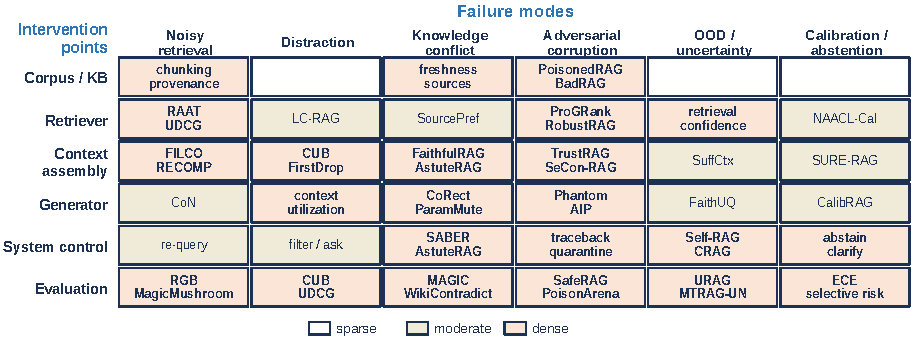
\includegraphics[width=\textwidth]{figures/generated/fig_failure_matrix.pdf}%
\caption{Schematic literature-family $\times$ intervention matrix. Shading and
example labels are illustrative design aids, not counts from Map~B;
quantitative Map-B distributions appear in Table~\ref{tab:corpus-stats}. Rows
are coordinate C3 and columns are coordinate C1, which is why a cell, not a
column, is the unit at which two systems become comparable.}
\label{fig:failure-intervention-matrix}
\end{figure*}

\begin{table*}[t]
\centering
\scriptsize
\renewcommand{\arraystretch}{0.92}
\begin{tabularx}{\linewidth}{>{\raggedright\arraybackslash}p{0.13\linewidth}>{\raggedright\arraybackslash}p{0.12\linewidth}>{\raggedright\arraybackslash}p{0.16\linewidth}>{\raggedright\arraybackslash}p{0.18\linewidth}>{\raggedright\arraybackslash}p{0.13\linewidth}>{\raggedright\arraybackslash}X}
\toprule
\textbf{Work} & \textbf{Failure} & \textbf{Task / setup} & \textbf{Key assumption} & \textbf{Metric} & \textbf{Boundary} \\
\midrule
IrrelCtx & irrelevant context & Open-domain QA & Irrelevance can be filtered or learned against & Robust accuracy & No adversarial/conflict setting. \\
RAAT & retrieval noise & Noisy QA training & Noise-aware training improves generation & F1/EM & Needs deployment-like noise. \\
RGB & multi-ability RAG & Bilingual benchmark & RAG reliability decomposes into abilities & Ability accuracy & Not adversarially adaptive. \\
FaithfulRAG & conflict & Fact-level conflict & Conflicts can be localised and reasoned over & Faithfulness & Needs reliable fact extraction. \\
AstuteRAG & imperfect retrieval & Training-free consolidation & Internal/external knowledge can be reliability-compared & Robust QA & Depends on LLM self-assessment. \\
PoisonedRAG & poisoning & Injected passages & Few crafted passages can dominate retrieval & Attack success & Targeted corruption focus. \\
RobustRAG & defense & Bounded corruption & Isolate-and-aggregate can certify robustness & Certificate, accuracy & Assumes attack budget. \\
Self-RAG / CtrlA & adaptive retrieval & Retrieve-or-answer & Model state can trigger retrieval & Trigger quality & Calibration can shift. \\
CalibRAG / URAG & calibration & Decision/MCQA & Confidence should reflect evidence uncertainty & ECE, coverage & Does not repair evidence. \\
PoisonArena / SafeRAG & security eval. & Poisoning benchmark & Threat models must be explicit & ASR, bypass & Still isolates attacks. \\
\bottomrule
\end{tabularx}
\caption{Analytical matrix of representative robust RAG work. Compared with a citation list, the matrix highlights each work's task setup, central assumption, metric focus, and boundary of applicability.}
\label{tab:analytical-matrix}
\end{table*}

\begin{table*}[t]
\centering
\scriptsize
\renewcommand{\arraystretch}{0.86}
\begin{tabularx}{\linewidth}{>{\raggedright\arraybackslash}p{0.13\linewidth}>{\raggedright\arraybackslash}p{0.17\linewidth}>{\raggedright\arraybackslash}p{0.17\linewidth}>{\raggedright\arraybackslash}p{0.16\linewidth}>{\raggedright\arraybackslash}p{0.13\linewidth}X}
\toprule
\textbf{Work} & \textbf{System setup} & \textbf{Failure construction} & \textbf{Metric / cost} & \textbf{Main claim} & \textbf{Failure boundary} \\
\midrule
IrrelCtx & RALM / open-domain QA; retrieved context injected into generator & Irrelevant passages with varying plausibility & Robust accuracy / answer degradation & Models can be brittle to irrelevant context. & Does not cover adversarial corruption or answerability policy. \\
RAAT & Noise-aware training for retrieval-augmented LMs & Multiple retrieval-noise types during training/evaluation & EM/F1 under noisy retrieval & Adaptive adversarial training improves noise robustness. & Transfer depends on whether deployment noise matches training noise. \\
RGB & Benchmark over English/Chinese QA-style RAG tasks & Noise, negative rejection, integration, counterfactual evidence & Ability-specific accuracy & RAG reliability decomposes into distinct abilities. & Benchmark abilities are diagnostic but not a unified control policy. \\
Sufficient Context & QA contexts labeled by sufficiency & Insufficient vs sufficient retrieved evidence & Selective answering / abstention quality & Evidence sufficiency should govern answerability. & Does not repair retrieval and does not model adversarial evidence. \\
PoisonedRAG & Corpus-injection attack against RAG & Crafted poisoned passages inserted into retrieval corpus & Attack success, retrieval of poison & Few poisoned documents can steer answers. & Strength depends on corpus write access, topic targeting, and retrieval success. \\
Certified / isolate defenses & Bounded-corruption RAG defense setting & Assumed corruption budget over retrieved evidence & Certificate, robust accuracy & Aggregation can certify robustness under budget assumptions. & Guarantees narrow when attacker violates budget or attacks instructions/tools. \\
Self-RAG / CtrlA & Adaptive retrieve-or-answer policies & Uncertainty about whether retrieval is needed & Trigger quality, answer utility, cost & Retrieval should be a conditional action. & Calibration shifts under distribution change; action cost often underreported. \\
RAGTruth & Annotated hallucination/faithfulness resource & Naturally generated unsupported spans across tasks & Span-level hallucination labels & Fine-grained support labels improve evaluation. & Faithfulness labels do not fully specify retrieval failure or system action. \\
\bottomrule
\end{tabularx}
\caption{Method-level comparison of representative robust-RAG work. The table makes explicit the setup, failure construction, metric target, main claim, and failure boundary that must be aligned before comparing methods.}
\label{tab:method-level-comparison}
\end{table*}


\begin{table*}[t]
\centering
\scriptsize
\renewcommand{\arraystretch}{0.86}
\begin{tabularx}{\linewidth}{>{\raggedright\arraybackslash}p{0.14\linewidth}>{\raggedright\arraybackslash}p{0.19\linewidth}>{\raggedright\arraybackslash}p{0.24\linewidth}>{\raggedright\arraybackslash}p{0.18\linewidth}X}
\toprule
\textbf{Case} & \textbf{Released rows / papers} & \textbf{Audited comparison fields} & \textbf{Metric or failure conflict} & \textbf{Synthesis / artifact boundary} \\
\midrule
Noise / distraction robustness & 5 rows: IrrelCtx, RAAT, Chain-of-Note, Sufficient Context, RGB & Assumption, QA dataset or benchmark slice, generator / reader setup, negative type, rank and gold-evidence availability. & EM/F1, rejection, selective risk, and ability-specific benchmark scores answer different questions. & Treat filtering, noise-aware training, generator reading, sufficiency prediction, and benchmark diagnosis as different mechanisms; artifact status is recorded per paper in the released worksheet. \\
Faithfulness, conflict, and attribution & 5 rows: RAGTruth, FaithfulRAG, AstuteRAG, Tug-of-War, Chain-of-Note & Unit of support, source-conflict assumption, attribution granularity, model-side reasoning setup, artifact availability. & Span-level support, fact-level conflict resolution, source preference, and final answer accuracy can disagree. & Citation faithfulness should not be collapsed into conflict robustness; the worksheet records where artifact evidence is dataset-level, code-level, or paper-only. \\
Adversarial corruption and RAG security & 6 rows: PoisonedRAG, corpus poisoning, BadRAG, certified defense, TrojanRAG, traceback & Corpus write access, insertion budget, retriever visibility, query control, generator access, stealth, retrieved malicious evidence, defense timing. & Attack success, certified robust accuracy, detection, traceback, and clean utility are not one defense score. & Compare only inside a capability envelope; prevention, demotion, detection, traceback, recovery, and certification remain separate outcomes. \\
Calibration, abstention, and adaptive control & 5 rows: Sufficient Context, Self-RAG, CRAG, CalibRAG, uncertainty RAG & Confidence target, evidence sufficiency labels, retrieval trigger, action set, cost budget, model/policy setup. & ECE, selective risk, coverage, retrieval-trigger quality, and answer utility can move in different directions. & Separate belief estimation from action selection; report coverage, cost, and final action alongside correctness. \\
Evaluation and benchmark comparability & 5 rows: RGB, RAGTruth, Sufficient Context, query robustness, RAG security benchmark & Evidence-state labels, perturbation source, model outputs scored, threat model, benchmark artifact availability. & Harder scores may reflect retrieval instability, unsupported spans, unanswerability, or adversarial steering. & Evaluation resources are diagnostic slices, not a universal robustness scale; benchmark comparisons require aligned evidence state and action policy. \\
\bottomrule
\end{tabularx}
\caption{Deeper case-study synthesis. The released 26-row worksheet compares assumptions, datasets or benchmark settings, model/evidence setup, metrics, failure modes, artifact availability, and comparison implications for the same five C1--C5 cases.}
\label{tab:deep-case-study-matrix}
\end{table*}

\begin{table*}[t]
\centering
\scriptsize
\renewcommand{\arraystretch}{0.9}
\begin{tabularx}{\linewidth}{>{\raggedright\arraybackslash}p{0.19\linewidth}>{\raggedright\arraybackslash}p{0.24\linewidth}>{\raggedright\arraybackslash}p{0.23\linewidth}X}
\toprule
\textbf{Apparent conclusion} & \textbf{What the framework changes} & \textbf{Non-trivial finding} & \textbf{Implication} \\
\midrule
``Method A is more robust to noise than method B.'' & Aligns noise type, rank position, gold-evidence availability, and intervention point. & Some methods solve generator distraction while others solve retriever defects; their scores are not competing estimates of the same property. & Report noise source and intervention point before ranking methods. \\
``Defense X lowers attack success.'' & Separates prevention, demotion, detection, traceback, and recovery. & A defense can improve traceback without lowering user-facing attack success, or certify bounded corruption without handling prompt-bearing documents. & Security papers should report outcome type, not only attack success rate. \\
``Calibration improves reliability.'' & Separates confidence in answer correctness from evidence sufficiency and action utility. & A calibrated answerer can still answer from insufficient evidence; an abstaining system can lower risk while reducing coverage. & Calibration metrics should be paired with evidence and action metrics. \\
``Benchmark Y is harder.'' & Compares evidence state, required action, cost budget, and metric target. & A benchmark can be hard because retrieval fails, because evidence conflicts, or because the correct action is refusal; these failures should not be pooled. & Leaderboards should expose diagnostic sub-scores instead of one robust-RAG score. \\
\bottomrule
\end{tabularx}
\caption{Distilled classes of non-trivial findings produced by the comparability framework. Main Table~\ref{tab:main-normalization-findings} gives the concrete paper-pair cases; this appendix table groups them into reusable interpretation rules.}
\label{tab:nontrivial-findings}
\end{table*}

\begin{table*}[t]
\centering
\scriptsize
\renewcommand{\arraystretch}{0.9}
\begin{tabularx}{\linewidth}{>{\raggedright\arraybackslash}p{0.24\linewidth}>{\raggedright\arraybackslash}p{0.25\linewidth}>{\raggedright\arraybackslash}p{0.21\linewidth}X}
\toprule
\textbf{Main claim} & \textbf{Cited evidence basis} & \textbf{What the evidence supports} & \textbf{Boundary} \\
\midrule
Irrelevant or noisy context can harm generation. & Irrelevant-context robustness, RAAT, RGB, and counterfactual-noise studies. & Noise affects both retrieval quality and generator context use. & Does not imply one robustness score covers all noise types. \\
Knowledge conflict differs from adversarial corruption. & Conflict and poisoning studies with different evidence origins and evaluation targets. & Natural disagreement and attacker-created contradiction require different assumptions. & Conflict-resolution results should not be read as poisoning-defense results. \\
RAG attacks require capability normalisation. & Poisoning, backdoor, prompt-injection, traceback, and certification studies. & Attack/defense results require corpus access, query control, retriever visibility, and budget. & The paper does not rank attacks by real-world prevalence. \\
Calibration, abstention, and retrieval control are distinct. & Sufficient-context, uncertainty, adaptive-retrieval, and calibration studies. & Confidence estimation, evidence sufficiency, retrieval triggering, and abstention optimise different quantities. & Does not validate a single universal control policy. \\
Action-trace evaluation is a benchmark agenda. & Benchmarks exposing subsets of answer, evidence, action, cost, and threat fields. & Existing benchmarks cover pieces of the proposed schema. & No new leaderboard or empirical system ranking is claimed. \\
\bottomrule
\end{tabularx}
\caption{Narrative claim-to-source ledger. Expanded and strict citation audits
were model-assisted and deterministic; this table records the intended evidence
boundary rather than certifying every citation.}
\label{tab:claim-verification-ledger}
\end{table*}


\subsection{Peer-Reviewed Backbone and Preprint Trends}

The main synthesis is anchored in the venue-linked backbone summarized in Table~\ref{tab:peer-reviewed-backbone}. Under that stricter evidence stratum, five conclusions remain stable: retrieved evidence can harm generation; conflict and poisoning require different assumptions; security results require attacker-capability normalization; calibration and abstention are separate control decisions; and answer accuracy alone is insufficient for robust-RAG evaluation. The broader 268-paper adjudicated map is still useful, but mainly for trend discovery and auditability. Its preprint-heavy cross-tabs are moved to Appendix~\ref{sec:map-statistics}; they diagnose where the map is dense or sparse, but they are not used as field-wide prevalence estimates.

\paragraph{Critical judgments from the re-analysis.}
The framework weakens three common readings of the literature. First, many ``robust to retrieval noise'' claims are over-broad: once distractor hardness, gold-evidence availability, and intervention point are aligned, several methods address complementary mechanisms rather than competing on one robustness axis. Second, many RAG security defenses are narrower than their abstracts suggest: a defense against bounded factual corruption is not evidence of robustness to prompt-bearing documents, trigger-based backdoors, or post-hoc traceback settings. Third, answer-only benchmark gains are often under-specified: without citation support, evidence sufficiency, and action-cost labels, a higher score can mean better answering, riskier coverage, or simply more computation. These are the places where the framework changes interpretation rather than merely renaming categories.

\subsection{Where Robustness Interventions Act}

Across the literature, robustness interventions cluster by where they act in the RAG pipeline. \textbf{Corpus-level interventions} sanitize, filter, watermark, or validate documents before indexing. They are attractive because they prevent bad evidence from entering the system, but they require corpus governance and may not be possible for open-web retrieval. \textbf{Retriever-level interventions} improve ranking, detect poisoned passages, or diversify evidence. They are efficient and model-agnostic, but they only control what enters the context, not how the generator uses it. \textbf{Context-level interventions} compress, reorder, or filter the retrieved context. They are flexible, but can remove qualifiers or multi-hop evidence. \textbf{Generator-level interventions} use prompting, fine-tuning, note-taking, self-reflection, or hidden-state control. They directly address evidence use but may be model-specific. \textbf{System-level interventions} decide when to retrieve, verify, abstain, or ask. They are closest to deployment needs but require calibrated signals from all earlier stages.

This intervention map helps explain why papers sometimes appear to solve the same problem while actually operating at different layers. For example, irrelevant-context filtering \citep{irrelevantContext2023}, Chain-of-Note \citep{chainOfNote2023}, and Sufficient Context \citep{sufficientContext2024} all address unreliable evidence, but the first filters evidence, the second changes generator reasoning, and the third changes answer policy. Similarly, PoisonedRAG-style attacks \citep{poisonedRAG2024} target the corpus-to-generation path, while AIP attacks prompt templates \citep{aip2025}. A comprehensive survey must therefore compare methods by intervention point, not only by reported task accuracy.

\subsection{Critical Case Studies of Taxonomy Use}
\begin{table*}[t]
\centering
\scriptsize
\renewcommand{\arraystretch}{0.9}
\begin{tabularx}{\linewidth}{>{\raggedright\arraybackslash}p{0.17\linewidth}>{\raggedright\arraybackslash}p{0.25\linewidth}>{\raggedright\arraybackslash}p{0.25\linewidth}X}
\toprule
\textbf{Case} & \textbf{Papers / settings compared} & \textbf{Why naive comparison fails} & \textbf{Synthesis from the framework} \\
\midrule
Noise / distraction robustness & IrrelCtx, RAAT, RGB, Chain-of-Note, Sufficient Context & Some vary retriever noise, some change generator reading behavior, and some decide answerability; robust accuracy, ability scores, and abstention metrics answer different questions. & Treat retrieval imperfection, harmful context influence, and insufficient evidence as separate states; compare methods only after fixing the intervention point and required action. \\
Faithfulness, conflict, and attribution & RAGTruth, FaithfulRAG, AstuteRAG, Tug-of-War, Chain-of-Note & Span-level support, fact-level conflict, document-level reading, and final answer correctness are different target objects. & Citation faithfulness is not the same as conflict robustness; valid comparisons must state support unit, source reliability assumption, and action policy. \\
Adversarial corruption and RAG security & PoisonedRAG, BadRAG, certified defenses, traceback methods, prompt-injection defenses & One result may assume corpus write access, another bounded corruptions, another instruction-bearing documents, and another post-hoc observability; attack success rates transfer poorly across assumptions. & Report corpus write access, insertion budget, retriever visibility, generator access, stealth, and whether malicious evidence was retrieved before comparing attacks or defenses. \\
Calibration, abstention, and adaptive control & Self-RAG, CRAG, CalibRAG, uncertainty RAG, Sufficient Context & ECE, selective risk, retrieval-trigger quality, and abstention precision measure different objects; better confidence does not necessarily repair evidence or choose the right user action. & Separate belief estimation from action selection. A complete benchmark should score confidence, evidence sufficiency, final action, and cost. \\
Evaluation and benchmark comparability & RGB, RAGTruth, Sufficient Context, query-robustness benchmarks, RAG security arenas & A benchmark can be hard because retrieval fails, evidence conflicts, attribution is unsupported, the item is unanswerable, or an attacker is stronger. & Evaluation resources should expose diagnostic sub-scores and threat/action labels rather than one robust-RAG scalar. \\
\bottomrule
\end{tabularx}
\caption{Critical case studies showing how the comparability framework changes interpretation of representative robust-RAG papers.}
\label{tab:critical-case-studies}
\end{table*}


\paragraph{Case 1: irrelevant evidence is not one problem.}
IrrelCtx, RAAT, RGB, Chain-of-Note, and Sufficient Context are sometimes all described as robustness-to-noise work, but they instantiate different experimental objects. IrrelCtx tests whether a generator can ignore irrelevant context; RAAT treats noise as a training distribution; RGB decomposes reliability into benchmark abilities; Chain-of-Note changes the generator's intermediate reading behavior; Sufficient Context changes the answer policy when evidence is inadequate. A direct leaderboard comparison would mix retrieval perturbation, generator selectivity, and answerability control. The taxonomy changes the question from ``which method is best under noise?'' to ``which evidence state is present, which module intervenes, and what action should be scored?''

\paragraph{Case 2: poisoning papers differ by attacker capability.}
Poisoning Retrieval Corpora, PoisonedRAG, BadRAG, TrojanRAG, Phantom, AIP, and newer one-shot or traceback studies are all adversarial, but they assume different access and objectives. Some manipulate dense retrieval, some steer final answers, some rely on triggers, some attack shared prompt templates, and some evaluate whether poisoned evidence can be traced after the fact. Attack success rate is therefore not a portable metric unless corpus write access, query control, retriever visibility, generator access, insertion budget, and stealth requirements are aligned. This is why Table~\ref{tab:attacker-capability} treats capability fields as part of the result, not just implementation detail.

\paragraph{Case 3: calibration is not the same as abstention.}
UncertaintyRAG, CalibRAG, URAG, Self-RAG, CtrlA, Sufficient Context, and SABER-style trust/abstain methods all relate to uncertainty, but they optimize different objects. Some estimate uncertainty in spans or answer sets; some calibrate decision confidence; some decide when to retrieve; some decide when to abstain; some predict whether the retrieved context is sufficient. Expected calibration error, selective risk, retrieval-trigger accuracy, and abstention precision cannot be collapsed into one number. The taxonomy forces a distinction between belief estimation and action selection, explaining why a method can improve calibration without repairing evidence or improve retrieval triggering without improving final answer faithfulness.

\paragraph{Case 4: poisoning defenses do not share one threat model.}
Certified defenses, isolate-and-aggregate defenses, poisoned-document detectors, activation-based traceback, and prompt-injection defenses respond to different adversarial assumptions. A certificate can be meaningful under a bounded corruption budget but irrelevant when the attacker controls prompt-like instructions; a traceback method may be useful after an incident but may not prevent answer steering; a prompt-injection defense may not address embedding-space poisoning. The framework therefore asks defense papers to report the same capability fields as attack papers and to distinguish prevention, detection, demotion, traceback, and recovery.

\subsection{Strengths and Weaknesses by Method Family}

Filtering and reranking are attractive robustness methods because they can be added around existing LLMs. Their weakness is false negatives: an aggressive filter may discard the only passage that supports a rare or multi-hop answer. Robust training can teach models to ignore noise, but training data may not cover future attacks or domain-specific distractors. Conflict modeling provides a principled way to handle contradictions, but fact extraction and alignment remain brittle for long, compositional, or numerical claims. Certified defenses provide valuable guarantees, but their assumptions are often narrower than realistic attack surfaces. Adaptive retrieval and abstention improve risk control, but their performance depends on calibration signals that can themselves be miscalibrated under distribution shift.

The synthesis suggests that method families should be composed according to risk profile rather than stacked indiscriminately. A low-risk FAQ system may only justify lightweight filtering and citation checks, while a high-stakes document-grounded setting may require source validation, contradiction detection, selective abstention, and escalation. These are design implications, not claims that the evidence map validates any particular enterprise, medical, or legal deployment.

\subsection{What Counts as Progress?}

The corpus currently reports progress through heterogeneous metrics: EM/F1, hallucination rate, retrieval recall, attack success rate, calibration error, abstention accuracy, and human preference. These metrics are not directly comparable. A defense that reduces attack success may reduce answer utility; a calibration method may improve selective risk while lowering coverage; a retriever that improves recall may increase distraction. Robust RAG progress should therefore be reported as a Pareto frontier across utility, robustness, calibration, cost, and security. This mirrors the broader lesson from trustworthy ML: robustness is not a scalar property but a tradeoff surface.

\subsection{What Is Still Missing from the Literature}

Several gaps recur across categories. First, benchmarks rarely combine failures. Noise, conflict, poisoning, and unanswerability are usually tested separately, even though realistic systems may encounter them jointly. Second, many papers evaluate with one retriever and one generator, making transfer difficult to assess. Third, few works evaluate long-term corpus dynamics: documents are updated, poisoned documents are removed, indices are rebuilt, and user feedback changes future retrieval. Fourth, most papers treat users as passive recipients rather than interactive participants who can clarify intent or verify sources. Fifth, multilingual and multimodal robust RAG remains underdeveloped relative to text-only English QA; because our corpus is also text-heavy, this is a boundary of the present survey rather than a resolved conclusion about those areas.

\section{Practical Guidelines}
\label{sec:guidelines}

The literature suggests different design priorities for different risk regimes, but the evidence base is strongest for text QA and document-grounded RAG. This section therefore gives design checklists and reporting guidance rather than validated deployment prescriptions for enterprise, medical, legal, or agentic systems.

\subsection{For Benchmark Builders}

Benchmark builders should avoid treating robustness as a single score. A useful benchmark should specify: (1) the corpus construction process; (2) the retriever and generator assumptions; (3) the failure type being tested; (4) whether failures are benign or adversarial; (5) the required system action; and (6) the cost budget. For noisy retrieval, benchmarks should vary the type and placement of distractors, not only the number of negative passages. For conflict, benchmarks should distinguish parametric--retrieved conflict from retrieved--retrieved conflict. For adversarial evaluation, benchmarks should report attacker knowledge, insertion budget, trigger type, and whether malicious evidence is actually retrieved. For uncertainty, benchmarks should include answerable, unanswerable, ambiguous, and underspecified questions.

Benchmarks should also provide evidence-level annotations. Without knowing which passage supports which claim, it is difficult to evaluate faithfulness or citation. Without knowing which passage is distracting, it is difficult to measure negative utility. Without knowing which document is poisoned, it is difficult to evaluate defense recall and false positives. The most useful future benchmarks will resemble diagnostic test suites rather than single leaderboard datasets.

\subsection{For Method Designers}

Method designers should state the intervention point. A method that filters retrieved passages should not be compared directly to a method that fine-tunes the generator unless the comparison controls for retriever, generator, corpus, and cost. A method that improves calibration should specify whether it calibrates answer correctness, evidence sufficiency, retrieval usefulness, or abstention. A method that handles knowledge conflict should specify whether it assumes retrieved evidence is more trustworthy than parametric memory.

Methods should also report failure cases. A filter may remove useful multi-hop evidence. A conflict resolver may over-trust internal knowledge when the model is outdated. A poisoning defense may fail against paraphrased or multimodal attacks. An abstention method may over-refuse when retrieval returns all-negative contexts. Reporting these failures is not merely a negative result; it clarifies the method's operating region and helps later work combine complementary methods.

\subsection{For System Builders}

System builders should start with risk assessment. If the corpus is closed, curated, and static, benign noise and calibration may dominate. If the corpus is open-web or user-editable, adversarial corruption becomes central. If the domain has high failure cost, answerability, provenance, and escalation should be first-class. If the system uses tools or persistent memory, retrieved instructions and memory poisoning require special controls. These recommendations are extrapolations from the surveyed text-RAG evidence and should be validated in the target domain.

A practical robust RAG stack should include at least four components. First, corpus governance: source tracking, ingestion filters, and update logs. Second, retrieval diagnostics: not just top-$k$ scores, but diversity, provenance, and conflict signals. Third, generation safeguards: evidence separation from instructions, claim-level support checks, and conflict-aware prompting or reasoning. Fourth, control policies: calibrated abstention, clarification, re-retrieval, and escalation. The exact implementation can be lightweight or heavy depending on risk, but the architecture should preserve these functions.

\section{Open Challenges and Future Directions}
\label{sec:future}

\paragraph{Unified evidence reliability estimation.}
Current systems often estimate relevance, faithfulness, safety, and confidence with separate modules. Robust RAG needs a unified evidence reliability model that accounts for relevance, sufficiency, consistency, provenance, freshness, and adversarial risk.

\paragraph{Causal understanding of context influence.}
We need better tools for measuring how each passage changes the final answer. Passage attribution, counterfactual context removal, hidden-state probing, and answer-flip analysis can help distinguish useful evidence from harmful distraction.

\paragraph{Conflict-aware generation.}
Fact-level conflict resolution remains immature. Future systems should explicitly represent claims, sources, timestamps, and confidence, and generate answers that expose unresolved conflict rather than hiding it.

\paragraph{Adaptive control under cost constraints.}
Retrieval, reranking, verification, and human review all have costs. Robust RAG should optimize risk--cost tradeoffs: when is extra retrieval worth it, when is abstention better, and when should a system ask the user for clarification?

\paragraph{Adversarially realistic benchmarks.}
Many attacks assume simplified access patterns, while many defenses assume narrow threat models. Benchmarks should specify attacker capabilities, corpus mutability, retriever visibility, access control, and deployment constraints.

\paragraph{Multimodal, agentic, and long-context RAG.}
Robustness becomes harder when evidence includes images, tables, code, web pages, memory, tools, or long-context documents. Agentic RAG introduces persistent memory and tool calls, expanding both the control problem and the attack surface.

\paragraph{Versioned evidence maps.}
The literature is changing quickly, especially around RAG attacks and defenses. The practical implication is modest but important: survey artifacts should be versioned and machine-readable. Our supplementary CSV files provide a first snapshot of paper categories, source strata, threat-model fields, benchmark dimensions, assumptions, and known limitations; maintaining a living survey would require public versioning, update cadence, and re-coding procedures beyond the scope of this submission.

\section{Limitations}
\label{sec:limitations}

The literature is evolving quickly, especially for RAG attacks and defenses. Some 2026 preprints may change before publication. Some metadata imported from public lists required manual cleaning, and some works appear in both preprint and proceedings form. The current taxonomy emphasizes text RAG and knowledge-intensive QA; multilingual, multimodal, code, tool-using, and agentic RAG are included where they directly affect robustness but are not yet treated exhaustively. Because we restrict collection to open PDFs, paywalled work may be underrepresented.

The corpus is source-skewed even after the venue-oriented pass: most reviewed records are arXiv preprints, while formally published venue-linked records are much smaller in count. This skew reflects both the rapid growth of RAG robustness preprints and our open-PDF collection strategy, but it limits claims about peer-reviewed coverage. The venue metadata pass and follow-up triage improve auditability but do not replace a manual venue-complete proceedings review over ACL, EMNLP, NAACL, COLING, SIGIR, WWW, WSDM, KDD, USENIX Security, CCS, NDSS, ICLR, and NeurIPS. The original 37 unprocessed venue-linked candidates have been triaged, but broader proceedings-level omissions may remain; hence we call the result a venue-augmented scoping set, not a venue-complete census.

The annotation evidence is stronger after round-2 human coding and final adjudication, but the survey remains a scoping review rather than a field census. The 274 candidate evidence records had strong human-human agreement before adjudication, and final adjudication produced a 268-paper evidence map. However, because the corpus is still open-PDF based and venue-augmented rather than venue-complete, category-overlap and method-family cross-tabs should be read as adjudicated map statistics rather than field prevalence estimates. These limitations are why the paper is framed as a structured scoping survey and framework proposal rather than an authoritative systematic review.

\section{Ethics and Dual-Use Considerations}
\label{sec:ethics}

This survey discusses attacks such as corpus poisoning, prompt injection, backdoors, opinion manipulation, and privacy extraction because they are central to understanding robust RAG. Such content is dual-use: detailed attack recipes can help defenders evaluate systems, but can also lower the barrier for misuse. We therefore present attacks at the level of threat model, failure mechanism, evaluation signal, and defense implication, rather than providing operational exploit prompts, payloads, or deployable attack code. We also pair attack discussions with defenses, assumptions, and responsible evaluation practices.

For benchmark builders and system developers, the ethical priority is to evaluate RAG systems without releasing harmful payloads, private data, or instructions that directly facilitate abuse. Poisoned documents used for evaluation should be synthetic or sandboxed, and benchmarks should avoid real personal data unless consent and privacy controls are explicit. For deployed systems, logs used for traceback or monitoring should follow data minimization, access control, and retention policies. Papers proposing new attacks should state disclosure plans, affected deployment assumptions, and whether released artifacts have been sanitized.

\section{Conclusion}

RAG is often presented as a solution to hallucination, but retrieval can also introduce new failure modes. This scoping survey treats robust RAG as an evidence-reliability and control problem: the central challenge is not only whether a system can retrieve evidence, but whether it can judge evidence reliability and choose the right action under uncertainty. The peer-reviewed and venue-linked backbone supports the mechanism-level conclusion that evidence failures, attacker assumptions, calibration targets, and action policies must be aligned before methods or benchmarks are compared. The broader adjudicated evidence map remains useful as a trend/audit artifact, not a field census. Within that boundary, robust RAG systems and benchmarks should evaluate not only whether the final answer is correct, but whether the system knows when evidence is unreliable, when to seek more evidence, when to ignore context, when to surface conflict, and when to abstain.

\appendix
\section{Current Core Reading List Sample}
\begin{table*}[t]
\centering
\scriptsize
\begin{tabularx}{\linewidth}{p{0.05\linewidth}X p{0.24\linewidth} p{0.10\linewidth}}
\toprule
Rank & Paper & Categories & Role \\
\midrule
1 & PoisonedRAG: Knowledge Corruption Attacks to Retrieval-Augmented Generation of Large Language Models & adv. corruption & attack \\
2 & Certifiably Robust RAG against Retrieval Corruption & adv. corruption & defense \\
3 & Making Retrieval-Augmented Language Models Robust to Irrelevant Context & noisy retrieval; distraction; calibration & method \\
4 & Enhancing Noise Robustness of Retrieval-Augmented Language Models with Adaptive Adversarial Training & noisy retrieval; evaluation & defense \\
5 & Phantom: General Backdoor Attacks on Retrieval Augmented Language Generation & adv. corruption & attack \\
6 & URAG: A Benchmark for Uncertainty Quantification in Retrieval-Augmented Large Language Models & OOD/uncertainty; calibration; evaluation; noise & benchmark \\
7 & Trust or Abstain? A Self-Aware RAG Approach & knowledge conflict; calibration; evaluation & method \\
8 & The First Drop of Ink: Nonlinear Impact of Misleading Information in Long-Context Reasoning & distraction; noisy retrieval & analysis \\
\bottomrule
\end{tabularx}
\caption{Sample entries from the core reading set. The full core set and metadata are provided in the supplementary material.}
\label{tab:core-sample}
\end{table*}


\section{Structured Evidence Map Sample}
\label{sec:lit-map}
\begin{table*}[t]
\centering
\scriptsize
\renewcommand{\arraystretch}{0.92}
\begin{tabularx}{\linewidth}{p{0.13\linewidth}p{0.12\linewidth}p{0.16\linewidth}p{0.15\linewidth}p{0.16\linewidth}X}
\toprule
\textbf{Paper} & \textbf{Year} & \textbf{Failure / risk} & \textbf{Method family} & \textbf{Intervention} & \textbf{Boundary / note} \\
\midrule
PoisonedRAG & 2025 & adversarial corruption & attack & corpus / KB & Targeted knowledge corruption; stealth and long-term dynamics vary. \\
RobustRAG & 2024 & adversarial corruption & defense & retriever / aggregation & Certification assumes bounded corruption. \\
IrrelCtx & 2023 & retrieval noise / distraction & defense & context filtering & Does not model adaptive attackers. \\
RAAT & 2024 & retrieval noise & training & generator & Requires deployment-like noisy training data. \\
FaithfulRAG & 2025 & knowledge conflict & conflict modeling & generator & Depends on fact extraction and alignment. \\
AstuteRAG & 2025 & imperfect retrieval + conflict & control / consolidation & system control & Relies on source-aware LLM self-assessment. \\
Self-RAG & 2024 & retrieval need & adaptive retrieval & system control & Retrieval trigger calibration can shift. \\
RGB & 2024 & multi-axis RAG failure & benchmark & evaluation & Not adversarially adaptive. \\
RAGTruth & 2024 & hallucination / faithfulness & benchmark & evaluation & Strong word-level labels, less retrieval-threat focus. \\
MTRAG-UN & 2026 & unanswerability & benchmark & system action & Multi-turn setting; security is secondary. \\
\bottomrule
\end{tabularx}
\caption{Sample of the structured evidence map. The full CSV supplement contains title, authors, year, source, taxonomy categories, failure/risk type, method family, intervention point, benchmark/task, metrics, contribution, and limitation/note for the cited literature map.}
\label{tab:evidence-map-sample}
\end{table*}



\section{Exploratory Map Statistics}
\label{sec:map-statistics}
\begin{table*}[t]
\centering
\small
\begin{tabularx}{\linewidth}{p{0.18\linewidth}X}
\toprule
\textbf{Dimension} & \textbf{Distribution in the 342-paper adjudicated Map B} \\
\midrule
Publication year & 2025: 170; 2024: 92; 2026: 65; 2023: 12; 2021: 2; 2022: 1 \\
Source / venue type & arXiv/preprint: 207; venue/proceedings-linked: 126; workshop/challenge: 5; other/unclear: 4 \\
Primary failure category & adversarial corruption: 120; knowledge conflict: 57; calibration/control: 55; evaluation/benchmark: 43; noisy retrieval: 34; distraction: 18; extension layer: 7; survey/background: 6; OOD/uncertainty: 2 \\
Method family & defense/mitigation: 119; attack: 75; benchmark/evaluation: 67; control/calibration: 27; method/evaluation: 21; analysis: 21; survey background: 6; conflict modeling: 4; method: 2 \\
Intervention point & generator: 81; corpus/KB: 67; evaluation: 51; context assembly: 48; mixed: 43; system control: 36; retriever/context: 15; not applicable: 1 \\
\bottomrule
\end{tabularx}
\caption{Descriptive corpus statistics for the canonical 342-row adjudicated Map B. These are map statistics, not field-wide prevalence estimates. Map A remains the IAA/adjudication snapshot.}
\label{tab:corpus-stats}
\end{table*}

\begin{table}[t]
\centering
\small
\begin{tabular}{lr}
\toprule
\textbf{Evidence stratum} & \textbf{Count} \\ 
\midrule
arXiv / preprint & 207 \\ 
venue / proceedings-linked & 126 \\ 
workshop / challenge & 5 \\ 
other / unclear & 4 \\ 
\bottomrule
\end{tabular}
\caption{Source strata in the canonical 342-row adjudicated Map B. Venue-linked coverage is now substantial relative to Map A, but the map remains a scoping corpus rather than a venue-complete census.}
\label{tab:evidence-strength}
\end{table}

\begin{table*}[t]
\centering
\scriptsize
\begin{tabular}{lrrrrrrrr}
\toprule
 & Noise & Distract & Conflict & Attack & OOD & Control & Eval. & Ext. \\ 
\midrule
Noise & 86 & 39 & 27 & 10 & 3 & 26 & 19 & 0 \\ 
Distract & 39 & 51 & 11 & 3 & 0 & 5 & 11 & 0 \\ 
Conflict & 27 & 11 & 104 & 22 & 5 & 20 & 34 & 1 \\ 
Attack & 10 & 3 & 22 & 135 & 1 & 10 & 21 & 0 \\ 
OOD & 3 & 0 & 5 & 1 & 40 & 34 & 10 & 0 \\ 
Control & 26 & 5 & 20 & 10 & 34 & 85 & 22 & 2 \\ 
Eval. & 19 & 11 & 34 & 21 & 10 & 22 & 90 & 1 \\ 
Ext. & 0 & 0 & 1 & 14 & 0 & 2 & 1 & 26 \\ 
\bottomrule
\end{tabular}
\caption{Category overlap in the 342-row adjudicated Map B. Extension-layer labels merge the historical \texttt{modality\_scenario} and \texttt{multimodal\_agentic\_code} names; counts are map diagnostics, not field prevalence.}
\label{tab:category-overlap}
\end{table*}

\begin{table*}[t]
\centering
\scriptsize
\begin{tabular}{lrrrrrrrr}
\toprule
\textbf{Method family} & Noise & Distract & Conflict & Attack & Control & Eval. & Ext. & Survey \\ 
\midrule
defense/mitigation & 27 & 12 & 33 & 37 & 9 & 0 & 1 & 0 \\ 
attack & 0 & 0 & 0 & 75 & 0 & 0 & 0 & 0 \\ 
benchmark/evaluation & 3 & 1 & 11 & 8 & 4 & 40 & 0 & 0 \\ 
control/calibration & 0 & 0 & 0 & 0 & 26 & 0 & 0 & 0 \\ 
method/evaluation & 3 & 1 & 1 & 0 & 8 & 2 & 6 & 0 \\ 
analysis & 1 & 4 & 8 & 0 & 6 & 1 & 0 & 0 \\ 
other/background & 0 & 0 & 4 & 0 & 2 & 0 & 0 & 6 \\ 
\bottomrule
\end{tabular}
\caption{Primary method-family by primary failure-type cross-tabulation over the 342-row adjudicated Map B. The table describes the map, not field-wide prevalence.}
\label{tab:method-failure-crosstab}
\end{table*}


\section{Detailed Audit Artifacts}
\label{sec:audit-artifacts}
\begin{table*}[t]
\centering
\small
\begin{tabularx}{\linewidth}{p{0.18\linewidth}p{0.16\linewidth}X}
\toprule
\textbf{Stage} & \textbf{Count} & \textbf{Rule} \\
\midrule
Initial retrieval & 1,904 records & Keyword search over arXiv, ACL Anthology, OpenReview, USENIX, AAAI/ACM landing pages where open versions were available, plus curated robust/trustworthy RAG paper lists; search cutoff 2026-06-03. \\
Open full-text corpus & 1,445 PDFs & Downloaded only open PDFs; removed failed downloads, inaccessible files, and non-PDF artifacts. \\
Deduplicated candidates & 1,399 papers & Deduplicated by normalised title and arXiv/proceedings identifiers; retained the most complete metadata record when preprint and proceedings versions overlapped. \\
Relevance screening & 536 included papers & Included papers that study RAG robustness, reliability, uncertainty, calibration, faithfulness, attack/defense, or evaluation under unreliable evidence; excluded application-only RAG papers. \\
Core pool & 112 papers & Papers directly shaping the taxonomy, threat/failure model, intervention mechanisms, or evaluation framework. \\
Core reading set & 100 papers & Core papers used as main narrative anchors; the remaining 12 core-pool papers stay in the broader scoping set. \\
Base scoping set & 300 papers & Core papers plus representative supporting work across all taxonomy branches before venue follow-up triage. \\
Venue-augmented scoping set & 326 papers & Base scoping set plus 26 venue-linked additions after follow-up triage. \\
Candidate evidence records & 274 papers & Base evidence map of 250 papers plus 24 venue-linked additions, double-coded and adjudicated. \\
Map A adjudicated seed & 268 papers & Candidate evidence records retained after final adjudication; used for IAA/adjudication provenance. \\
Map-B candidate expansion & 416 papers & Map A plus 148 source-blind human-citation-audit additions and 20 enriched original rows; used for second-coding review. \\
Map B adjudicated synthesis map & 342 papers & Map A plus 74 retained additions after second coding and final adjudication; frozen for current descriptive statistics. Post-freeze discoveries enter a recall log until a new version is coded. \\
\bottomrule
\end{tabularx}
\caption{Screening-flow summary. Search ends on 2026-06-03; coding and adjudication artifacts freeze on 2026-06-15. The supplement provides query strings, source counts, rules, exclusions, hashes, and a post-freeze recall log.}
\label{tab:review-protocol}
\end{table*}

\begin{table*}[t]
\centering
\scriptsize
\renewcommand{\arraystretch}{0.92}
\begin{tabularx}{\linewidth}{>{\raggedright\arraybackslash}p{0.17\linewidth}>{\raggedleft\arraybackslash}p{0.07\linewidth}>{\raggedright\arraybackslash}p{0.24\linewidth}X}
\toprule
\textbf{Set} & \textbf{N} & \textbf{Audit artifact} & \textbf{Selection rule and role} \\
\midrule
Retrieved records & 1,904 & \texttt{search\_protocol.json} & Initial keyword and curated-list retrieval before PDF availability, deduplication, or relevance screening. \\
Open full-text PDFs & 1,445 & \texttt{pdfs/} & Records with open PDFs available for full-text inspection; inaccessible or non-PDF artifacts removed. \\
Deduplicated candidates & 1,399 & \texttt{all\_reviewed\_deduped.csv} & Normalized-title and identifier deduplication; one record retained for preprint/proceedings overlaps. \\
Relevant included papers & 536 & \texttt{all\_reviewed\_deduped.csv} & Papers with decision \texttt{core} (112) or \texttt{include} (424); background-adjacent papers (289) and excluded papers (574) are tracked separately. \\
Core pool & 112 & \texttt{decision=core} in \texttt{all\_reviewed\_deduped.csv} & Papers judged central to taxonomy, threat/failure models, intervention mechanisms, or evaluation design. \\
Core reading set & 100 & \texttt{core100\_full.csv} & Main narrative anchors. The 12 core-pool papers not in this set remain in the base scoping set rather than being discarded. \\
Base scoping set & 300 & \texttt{survey300\_full.csv} & Core pool plus representative supporting work across failure categories, method families, and evaluation settings before venue follow-up triage. \\
Venue-augmented scoping set & 326 & \texttt{survey\_set\_venue\_audited.csv} & Base scoping set plus 26 venue-linked papers added after follow-up triage. \\
Base evidence map & 250 & \texttt{evidence\_map.csv} & Original structured map used before venue follow-up triage. \\
Candidate evidence records & 274 & round2 full adjudication CSV & Base map plus venue-linked additions, double-coded by humans and adjudicated. \\
Map A adjudicated seed & 268 & \texttt{evidence\_map\_adjudicated.csv} & Candidate evidence records with final \texttt{include\_in\_evidence\_map=1}; used for IAA/adjudication provenance. \\
Source-blind citation audit & 300 & \texttt{citation\_annotations.csv} & Source-blind human citation decisions over the venue and extension pools; distinct from the base scoping set. \\
Map-B candidate expansion & 416 & candidate expansion CSV & Map A plus 148 candidate additions supported by the source-blind citation audit and 20 enriched original rows; used for second coding. \\
Map B adjudicated synthesis map & 342 & adjudicated Map-B CSV & Map A plus 74 retained additions after second-coding adjudication; used for current synthesis statistics. \\
\bottomrule
\end{tabularx}
\caption{Corpus-set ledger. Exact memberships are released as CSV files for Map A, the 416-row candidate expansion, and the 342-row adjudicated Map B.}
\label{tab:set-selection-ledger}
\end{table*}

\begin{table*}[t]
\centering
\scriptsize
\renewcommand{\arraystretch}{0.94}
\begin{tabularx}{\linewidth}{>{\raggedright\arraybackslash}p{0.18\linewidth}>{\raggedright\arraybackslash}p{0.23\linewidth}>{\raggedright\arraybackslash}p{0.24\linewidth}X}
\toprule
\textbf{Artifact / claim source} & \textbf{Verification performed} & \textbf{What is coding- or metadata-assisted} & \textbf{How it is used in the paper} \\
\midrule
Main narrative claims and central citations & Author inspection of full paper text for papers used to support central claims, tables, and figures. & Initial prioritization and category suggestions were LLM-assisted. & Used for qualitative synthesis and case-study comparisons. \\
Core reading set & 100 papers curated from the 112-paper core pool after full-text relevance checks for narrative fit. & Core-pool creation used relevance scores and pre-labels as triage signals. & Used as the main reading backbone; not claimed to be a reproducible top-100 ranking without author judgment. \\
Map A, 268-paper adjudicated seed & Metadata and structured fields manually cleaned; venue-candidate triage completed; 274 candidate records independently double-coded and adjudicated into 268 included evidence-map papers. & Initial candidate discovery and pre-labeling were LLM-assisted, but final Map-A labels use human adjudication for coder disagreements. & Used for IAA/adjudication provenance, with the caveat that it is not the current synthesis denominator. \\
Map-B candidate expansion, 416 rows & Map A merged with source-blind human citation audit over the venue/extension pools; 148 new candidate rows added and 20 original rows enriched. & Candidate additions use human citation-audit decisions and deterministic field completion before second coding. & Used as the candidate pool for second coding, not as the final synthesis denominator. \\
Map B, 342-paper adjudicated synthesis map & Two coders independently second-coded all 148 additions; final adjudication retained 74 and excluded 74. & The retained additions use adjudicated labels; excluded boundary rows remain available in the release package. & Used for current source-stratified synthesis and venue sensitivity; still not a field census. \\
Human double-coding package & Two anonymized human sources independently coded all 274 candidate evidence records before discussion; round-2 agreement is strong across taxonomy, intervention, evidence-strength, relevance, core, and inclusion fields. & Disagreements were resolved in the final adjudication file. & Used to report pre-adjudication IAA and produce final adjudicated evidence-map labels. \\
Venue metadata pass and triage & ACL Anthology title/abstract scan plus DBLP/OpenAlex query logs, title matching, and follow-up triage decisions. & Discovery is metadata-based; inclusion/exclusion decisions are author triage rather than independent double coding. & Used to update venue-linked coverage and quantify remaining systematic-review limits. \\
\bottomrule
\end{tabularx}
\caption{Verification and annotation provenance. The table separates full-text author inspection, coding-assisted labels, metadata-derived venue candidates, and non-adjudicated consistency diagnostics.}
\label{tab:verification-provenance}
\end{table*}

\begin{table*}[t]
\centering
\scriptsize
\renewcommand{\arraystretch}{0.9}
\begin{tabularx}{\linewidth}{>{\raggedright\arraybackslash}p{0.19\linewidth}>{\raggedright\arraybackslash}p{0.25\linewidth}>{\raggedright\arraybackslash}p{0.24\linewidth}X}
\toprule
\textbf{Item} & \textbf{What was done} & \textbf{What was hidden from annotators} & \textbf{What we do not claim} \\
\midrule
Round-2 coders & Two anonymized coding-source records cover the same 274 candidate evidence records. & Machine pre-labels, prior evidence-map labels, previous adjudication logs, and the other source's labels. & The public package does not establish qualifications or personnel overlap; we claim file-level provenance, not independently verified expertise. \\
Training / codebook & Coders used the double-coding protocol and codebook defining scope, legacy literature-family tag, method family, intervention point, evidence strength, and inclusion fields. & Prior LLM rationales and model confidence scores. & We do not claim the codebook is final for all RAG subareas; adjudication notes can still motivate revisions. \\
Pre-adjudication separation & IAA was computed from separately completed CSV files before adjudication. & Post-discussion labels were not used for IAA. & This establishes workflow separation in the files, not personnel independence beyond the anonymized records. \\
Adjudication & A final adjudication file resolved 469 field-level disagreements and produced the 268-paper Map-A seed. & Source labels were preserved and not overwritten. & We do not apply Map-A IAA to the 148 later Map-B additions. \\
Source-blind citation audit & One source-blind citation-audit record set coded 300 papers from the venue/extension pools; 168 audited rows entered or enriched Map B after de-duplication and relevance checks. & Paper IDs were source-normalised and the audit did not use Map-A disagreement labels. & We do not claim 416-row double-coding, inter-annotator agreement, or independently verified annotator provenance for this batch. \\
\bottomrule
\end{tabularx}
\caption{Annotation transparency for the coding round. The table distinguishes file-auditable workflow separation from qualifications and personnel independence that the blind package does not establish.}
\label{tab:annotation-transparency}
\end{table*}

\begin{table*}[t]
\centering
\scriptsize
\begin{tabularx}{\linewidth}{p{0.24\linewidth}p{0.14\linewidth}p{0.14\linewidth}X}
\toprule
\textbf{Field} & \textbf{Agreement} & \textbf{$\kappa$ / score} & \textbf{Interpretation} \\
\midrule
Full-text checked & 100.0\% & 1.00 & Both sources marked every evidence-map paper as full-text checked. \\
In-scope screening & 99.6\% & 0.92 & Near-complete agreement; only one screening disagreement remains for adjudication. \\
Relevance level & -- & 0.80 & Linear-weighted agreement is strong for exclude/background/support/core priority. \\
Primary failure type & 97.1\% & 0.96 & Very strong human agreement on the main taxonomy category. \\
Method family & 89.4\% & 0.86 & Strong agreement on attack, benchmark, control, method, and analysis families. \\
Intervention point & 93.4\% & 0.92 & Very strong agreement on pipeline placement. \\
Evaluation type & 94.9\% & 0.93 & Very strong agreement on metric/evaluation family. \\
Evidence strength & 97.8\% & 0.95 & Very strong agreement on proceedings/preprint/review-platform strata. \\
Core-candidate decision & 91.6\% & 0.80 & Strong agreement on whether papers should shape the core narrative. \\
Include in evidence map & 99.3\% & 0.85 & Strong agreement on evidence-map inclusion. \\
Secondary labels & 79.2\% exact & 0.83 Jaccard & Multilabel agreement is strong enough to support overlap analysis after adjudication. \\
Reproducibility evidence & 10.6\% exact & 0.20 Jaccard & Weak free-text agreement; retained as adjudicated audit metadata, not used for primary comparison or trend claims. \\
\bottomrule
\end{tabularx}
\caption{Round-2 human-human agreement on 274 candidate evidence records before adjudication. Structured labels show strong agreement, while the free-text reproducibility field is weak and is treated only as adjudicated audit metadata. Two anonymized human annotation sources independently coded the same records; remaining disagreements were resolved to produce the 268-row Map-A adjudicated seed. These IAA values do not apply to the 148 later Map-B additions.}
\label{tab:iaa}
\end{table*}

\begin{table*}[t]
\centering
\scriptsize
\renewcommand{\arraystretch}{0.94}
\begin{tabularx}{\linewidth}{>{\raggedright\arraybackslash}p{0.22\linewidth}>{\raggedright\arraybackslash}p{0.24\linewidth}>{\raggedright\arraybackslash}p{0.20\linewidth}X}
\toprule
\textbf{Claim} & \textbf{Status under venue-linked / peer-reviewed evidence} & \textbf{What changes without preprints} & \textbf{Interpretation} \\
\midrule
Retrieved evidence can harm generation even when relevant evidence exists. & Holds: supported by venue-linked work on irrelevant/noisy context, noise-robust training, counterfactual noise, and imperfect retrieval. & The range of stress-test variants shrinks. & This is a stable mechanism-level claim. \\
RAG security results require attacker-capability normalisation. & Holds partially: venue-linked security work covers poisoning, traceback, membership inference, and backdoor-style corpus attacks. & Many fine-grained attack variants and defenses remain preprint-heavy. & The capability matrix is stable; detailed landscape counts are emerging trends. \\
Calibration, abstention, and retrieval control are distinct decisions. & Holds conceptually with venue-linked answerability, relevance-assessment, and calibration/control papers. & Specific method rankings and benchmark prevalence become sparse. & The conceptual separation remains; empirical prevalence is not settled. \\
The evidence map is attack- and benchmark-heavy. & Does not become a field-wide claim. & Under peer-reviewed-only evidence, the sample is much smaller and more evaluation-heavy. & Treat distributional cross-tabs as corpus diagnostics, not prevalence estimates. \\
Action-trace benchmark blueprint should score answer, evidence state, action, and cost. & Supported as a design synthesis, not validated as a benchmark standard. & The proposal becomes less empirical and more normative. & Keep as a research agenda unless a full benchmark is built and evaluated. \\
\bottomrule
\end{tabularx}
\caption{Peer-reviewed / venue-linked sensitivity analysis. The table states which conclusions survive when preprint-only evidence is downweighted and which remain hypothesis-generating.}
\label{tab:peer-reviewed-sensitivity}
\end{table*}


\begin{table*}[t]
\centering
\scriptsize
\renewcommand{\arraystretch}{0.94}
\begin{tabularx}{\linewidth}{>{\raggedright\arraybackslash}p{0.20\linewidth}>{\raggedright\arraybackslash}p{0.25\linewidth}>{\raggedright\arraybackslash}p{0.18\linewidth}X}
\toprule
\textbf{Pass} & \textbf{Scope} & \textbf{Observed yield} & \textbf{Interpretation} \\
\midrule
ACL Anthology metadata scan & ACL, EMNLP, NAACL, COLING; 2020--2026; full anthology BibTeX with abstracts & 12,924 entries scanned; 181 RAG candidates; 30 robust-RAG candidates & A reproducible proceedings-level metadata scan for core NLP venues, not just backfilled metadata. \\
DBLP/OpenAlex metadata queries & 15 robust-RAG query strings over venue-linked metadata for SIGIR, WWW, WSDM, KDD, USENIX Security, CCS, NDSS, ICLR, NeurIPS and overlaps & 31 query rows; 51 unique venue-linked candidate titles after deduplication & Surfaced missing venue-linked candidates; all 51 were subsequently triaged. \\
Follow-up venue triage & 51 venue-linked candidates & 23 new evidence-map additions; 3 background additions; 9 exclusions; 2 duplicates; 13 already represented & Closes the unprocessed venue-candidate gap, while still not claiming complete manual proceedings coverage. \\
Map A adjudicated seed & 268 evidence-map papers & 42 venue/proceedings-linked; 222 arXiv-only or emerging preprints; 4 other strata & IAA/adjudication basis before venue expansion. \\
Map-B candidate expansion & 416 evidence-map candidates & 194 venue/proceedings-linked; 207 arXiv/preprint; 11 workshop/challenge; 4 other/unclear & Pre-adjudication candidate map after source-blind citation audit. \\
Map B adjudicated synthesis map & 342 evidence-map papers & 126 venue/proceedings-linked; 207 arXiv/preprint; 5 workshop/challenge; 4 other/unclear & Current source-stratified synthesis map after second coding and final adjudication. \\
\bottomrule
\end{tabularx}
\caption{Venue-oriented search, coverage audit, and follow-up triage summary. Full query logs, candidate titles, decisions, and limitations are in \texttt{venue\_systematic\_queries.csv}, \texttt{venue\_systematic\_candidates.csv}, \texttt{venue\_coverage\_audit.csv}, and \texttt{venue\_triage\_decisions.csv}.}
\label{tab:venue-pass-summary}
\end{table*}

\begin{table*}[t]
\centering
\scriptsize
\renewcommand{\arraystretch}{0.94}
\begin{tabularx}{\linewidth}{>{\raggedright\arraybackslash}p{0.20\linewidth}>{\raggedright\arraybackslash}p{0.18\linewidth}>{\raggedright\arraybackslash}p{0.18\linewidth}X}
\toprule
\textbf{Coverage check} & \textbf{Count} & \textbf{Artifact} & \textbf{Interpretation} \\
\midrule
Venue-linked robust-RAG candidates found by metadata pass & 51 unique titles & candidate CSV & Candidate pool from ACL Anthology, DBLP, and OpenAlex metadata queries. \\
Already in core100 & 6 / 51 & coverage audit CSV & Core narrative captures only a small subset of venue-linked candidates. \\
Already in base scoping set & 14 / 51 & coverage audit CSV & The current scoping set misses or intentionally excludes many venue-linked candidates. \\
Already in evidence map & 13 / 51 & coverage audit CSV & Cross-tabs should be interpreted as map statistics, not field statistics. \\
Not in original base scoping set & 37 / 51 & coverage audit CSV & These papers were subsequently triaged; see Table~\ref{tab:venue-triage-summary}. \\
\bottomrule
\end{tabularx}
\caption{Venue-coverage audit after the metadata pass. The audit quantifies residual coverage risk by matching venue-linked candidates against the original core, survey, and evidence-map sets. Files: \texttt{venue\_systematic\_candidates.csv} and \texttt{venue\_coverage\_audit.csv}.}
\label{tab:venue-coverage-audit}
\end{table*}

\begin{table*}[t]
\centering
\scriptsize
\renewcommand{\arraystretch}{0.9}
\begin{tabularx}{\linewidth}{>{\raggedright\arraybackslash}p{0.20\linewidth}>{\raggedright\arraybackslash}p{0.24\linewidth}>{\raggedright\arraybackslash}p{0.20\linewidth}X}
\toprule
\textbf{Recall check} & \textbf{Observed result} & \textbf{What it controls} & \textbf{Residual risk} \\
\midrule
ACL Anthology metadata scan & 12,924 entries scanned for ACL/EMNLP/NAACL/COLING; 181 RAG candidates; 30 robust-RAG candidates & Reduces reliance on arXiv-only discovery for core NLP venues. & Title/abstract terms can miss papers using older QA/IR terminology. \\
Cross-venue metadata pass & DBLP/OpenAlex queries yielded 51 venue-linked robust-RAG candidates & Adds IR, web, security, and ML venue-linked records. & API ranking, metadata naming, and transient query errors limit recall. \\
Follow-up triage & 51 candidates triaged; 26 added to scoping set; 24 added to evidence map; 9 excluded; 2 duplicates & Closes the known unprocessed venue-candidate gap. & Does not prove complete coverage of every proceedings volume. \\
Evidence-strength sensitivity & Main conclusions separated into venue-linked backbone vs preprint trend evidence & Prevents preprint-heavy map statistics from becoming field-level claims. & Some emerging security/control subtopics remain too new for strong consensus. \\
\bottomrule
\end{tabularx}
\caption{Venue-recall risk analysis. The venue pass improves auditability and adds missed venue-linked papers, but it is still not a manual venue-complete proceedings review.}
\label{tab:venue-recall-risk}
\end{table*}


\begin{table*}[t]
\centering
\scriptsize
\renewcommand{\arraystretch}{0.94}
\begin{tabularx}{\linewidth}{>{\raggedright\arraybackslash}p{0.22\linewidth}>{\raggedright\arraybackslash}p{0.15\linewidth}>{\raggedright\arraybackslash}p{0.20\linewidth}X}
\toprule
\textbf{Triage outcome} & \textbf{Count} & \textbf{Action} & \textbf{Reasoning} \\
\midrule
Already represented in base evidence map & 13 & retain & Candidate was already included; metadata pass only improved venue visibility. \\
New evidence-map additions & 23 & add to evidence extension & Directly studies robust RAG, RAG evaluation, evidence reliability, security, calibration, or robust generation. \\
Scoping-set paper promoted to evidence extension & 1 & add to evidence extension & Already in the scoping set but not the base map; venue audit identified it as relevant to trust/calibration. \\
Background additions & 3 & add to venue-augmented scoping set only & Relevant boundary papers on domain, multilingual, or multimodal RAG, but not central text evidence-reliability evidence. \\
Excluded false positives / applications & 9 & exclude with reason & Application or adjacent RAG papers without robustness/evidence-reliability analysis. \\
Duplicate venue records & 2 & deduplicate & Same work already represented through another metadata record. \\
\midrule
\textbf{Venue-augmented scoping set} & \textbf{326} & base 300 + 26 additions & Updated scoping set after follow-up triage. \\
\textbf{Map A adjudicated seed} & \textbf{268} & 274 candidates - 6 exclusions & IAA/adjudication snapshot after human adjudication of double-coded candidate evidence records. \\
\textbf{Map-B candidate expansion} & \textbf{416} & Map A + 148 citation-audit-supported additions & Pre-adjudication candidate map after source-blind citation audit. \\
\textbf{Map B adjudicated synthesis map} & \textbf{342} & Map A + 74 retained additions & Current evidence map for synthesis after second coding and adjudication. \\
\bottomrule
\end{tabularx}
\caption{Follow-up triage of all 51 venue-linked candidates from the metadata pass. The 37 candidates outside the original scoping set are no longer unprocessed; decisions and reasons are in \texttt{venue\_triage\_decisions.csv}.}
\label{tab:venue-triage-summary}
\end{table*}

\begin{table*}[t]
\centering
\scriptsize
\begin{tabularx}{\linewidth}{p{0.18\linewidth}p{0.42\linewidth}X}
\toprule
\textbf{Category} & \textbf{Definition} & \textbf{Inclusion rule} \\
\midrule
Noisy retrieval & Benign retrieval imperfection: irrelevant passages, hard negatives, missing positives, stale or low-quality evidence. & Explicitly analyzes or mitigates retrieval noise, not merely uses retrieval. \\
Distraction & Retrieved context has negative marginal utility and changes answer, confidence, or reasoning despite not supporting the answer. & Includes distractor, context-utilization, or long-context degradation analysis. \\
Knowledge conflict & Contradiction between parametric knowledge and retrieved evidence, or among retrieved sources. & Includes conflict detection, source preference, fact-level reconciliation, or contextual faithfulness. \\
Adversarial corruption & Adaptive attacker manipulates corpus, retriever, prompt template, retrieved context, memory, or tools. & Includes poisoning, prompt injection, backdoors, attack/defense benchmarks. \\
OOD / uncertainty & Query or evidence is ambiguous, underspecified, unanswerable, out-of-knowledge-base, or under distribution shift. & Includes answerability, uncertainty quantification, or selective prediction. \\
Calibration / control & System decides when to retrieve, trust evidence, answer, abstain, clarify, or escalate. & Includes adaptive retrieval, calibrated decision-making, or abstention. \\
Evaluation benchmark & Paper introduces benchmark, dataset, metric, or evaluation protocol for robust RAG. & Must define evaluation axis, data, perturbation/threat, or metric. \\
\bottomrule
\end{tabularx}
\caption{Taxonomy codebook used for paper categorization. The full codebook is provided in the supplementary material.}
\label{tab:codebook}
\end{table*}


\bibliography{references,auto_references}

\end{document}
